\documentclass[12pt]{article}

\usepackage[utf8]{inputenc}
\usepackage{graphicx}
\usepackage{geometry}
\usepackage{hyperref}
\usepackage{listings}
\usepackage{color}
\usepackage{xcolor}
\usepackage{float}
\usepackage{tabulary}
\usepackage{enumitem}

% Page setup
\geometry{a4paper, margin=1in}

% Code listing setup
\lstset{
    basicstyle=\ttfamily\small,
    breaklines=true,
    postbreak=\mbox{\textcolor{red}{$\hookrightarrow$}\space},
    backgroundcolor=\color{gray!10},
    frame=single
}   

\begin{document}

\begin{titlepage}
    \centering

    \vspace*{1cm}

    \rule{\textwidth}{1pt}

    \vspace{2\baselineskip}

    {\huge  Cyber Security } \\

    \vspace{1\baselineskip}

    {\huge \textbf{ SIS: Firewall/Hash/Port Scanner }}

    \vspace{2\baselineskip}

    \rule{\textwidth}{1pt}

    \vspace{1cm}

    \large

    \begin{flushleft}
        \begin{minipage}{.8\textwidth}
            \raggedright
            Fullname: Amangeldi Zhanserik \\
            ID: 22B030301 \\
            E-mail: {\normalsize \url{zha_amangeldi@kbtu.kz}} \\
            Date of submission: \today \\
            Class time: Thursday, 15:00--18:00 \\
        \end{minipage}%
    \end{flushleft}

    \vspace{2cm}

    
\includegraphics[width=.7\textwidth]{logo-kbtu.png}

    \vfill

    School of Information System and Engineering \\
    Kazakh-British Technical University \\
    Academic Year 2024-2025 \\
\end{titlepage}

\tableofcontents
\newpage

\section{Lab 1: Configuring a Firewall}

\subsection{Objective}
In this lab, I worked with Linux firewall configurations using iptables. The main objectives were:
\begin{itemize}
    \item Installing and configuring an Apache web server
    \item Managing firewall rules with iptables to control HTTP traffic
    \item Analyzing firewall logs to understand connection attempts
\end{itemize}

\subsection{Key Steps and Observations}

\subsubsection{Installing and Starting Apache Server}
I installed Apache on the Security Workstation using the following commands:

\begin{lstlisting}
sudo apt update
sudo apt install apache2 -y
sudo systemctl start apache2
sudo systemctl enable apache2
\end{lstlisting}
After installation, I verified the server was active by checking its status:

\begin{figure}[H]
    \centering
    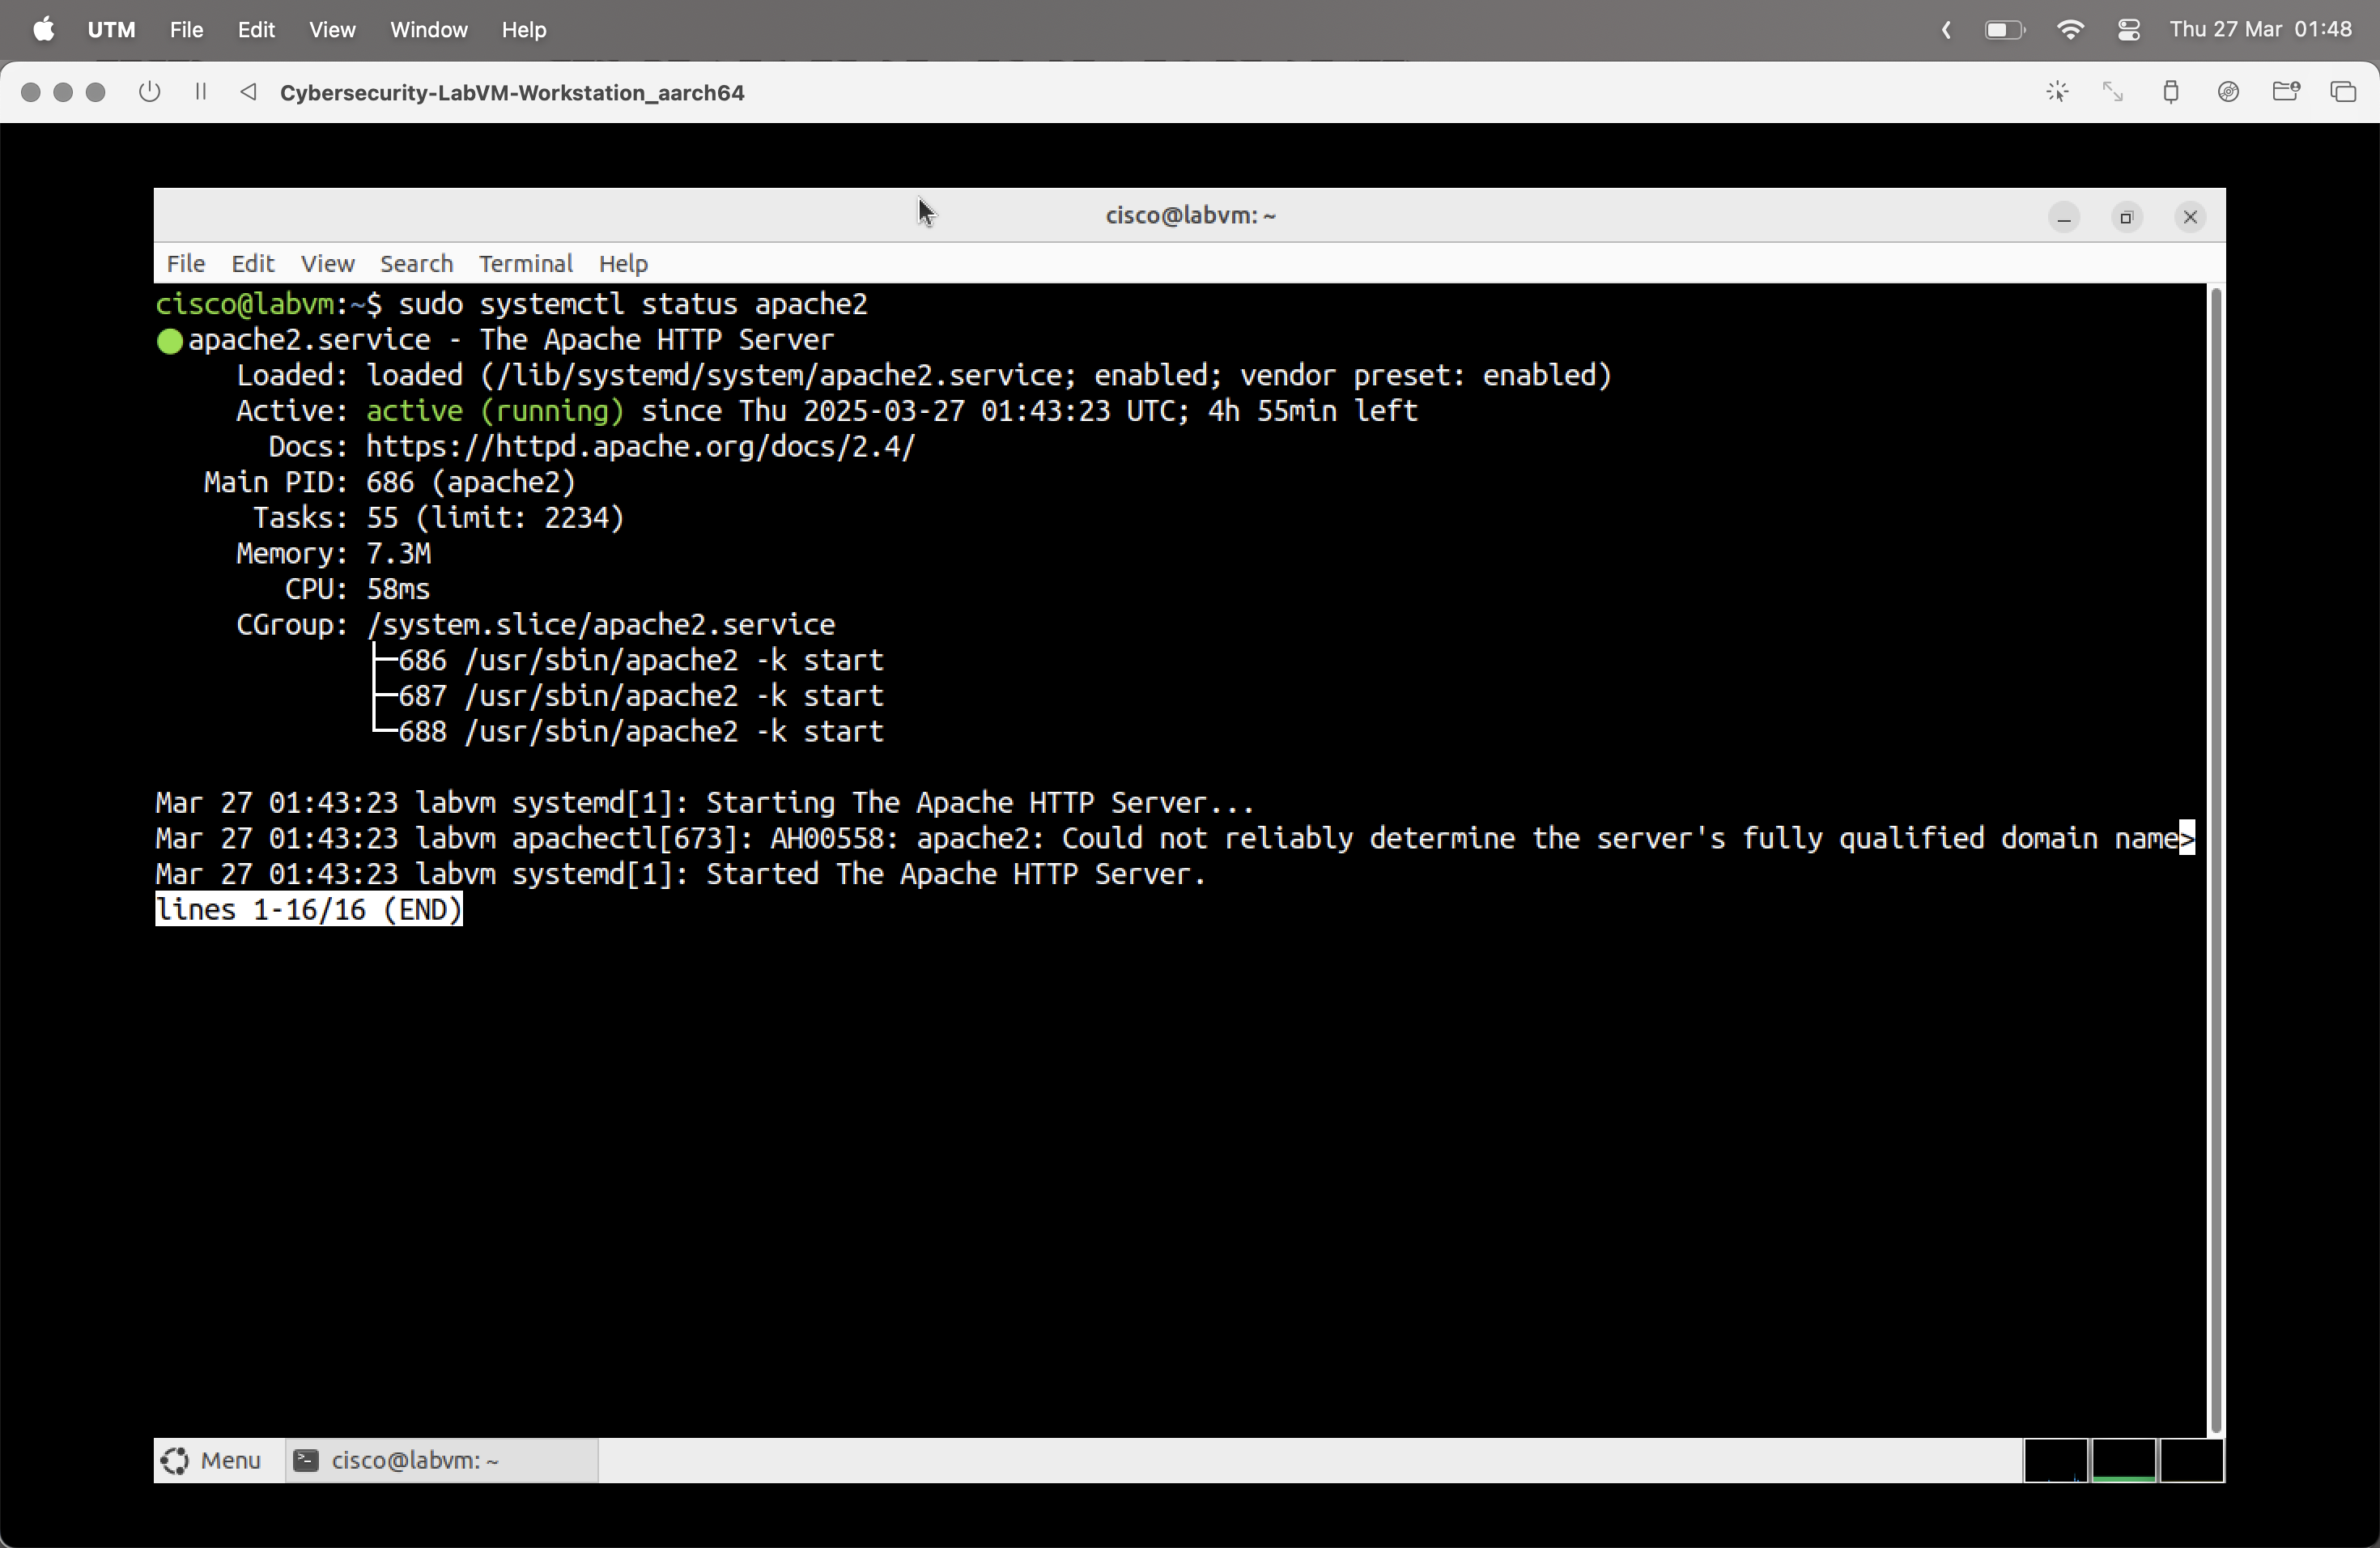
\includegraphics[width=0.8\textwidth]{lab1_apache_status.png}
    \caption{Apache server status showing active}
\end{figure}

\newpage

The IP address of my VM was determined to be: \textbf{172.18.1.45}

\begin{figure}[H]
    \centering
    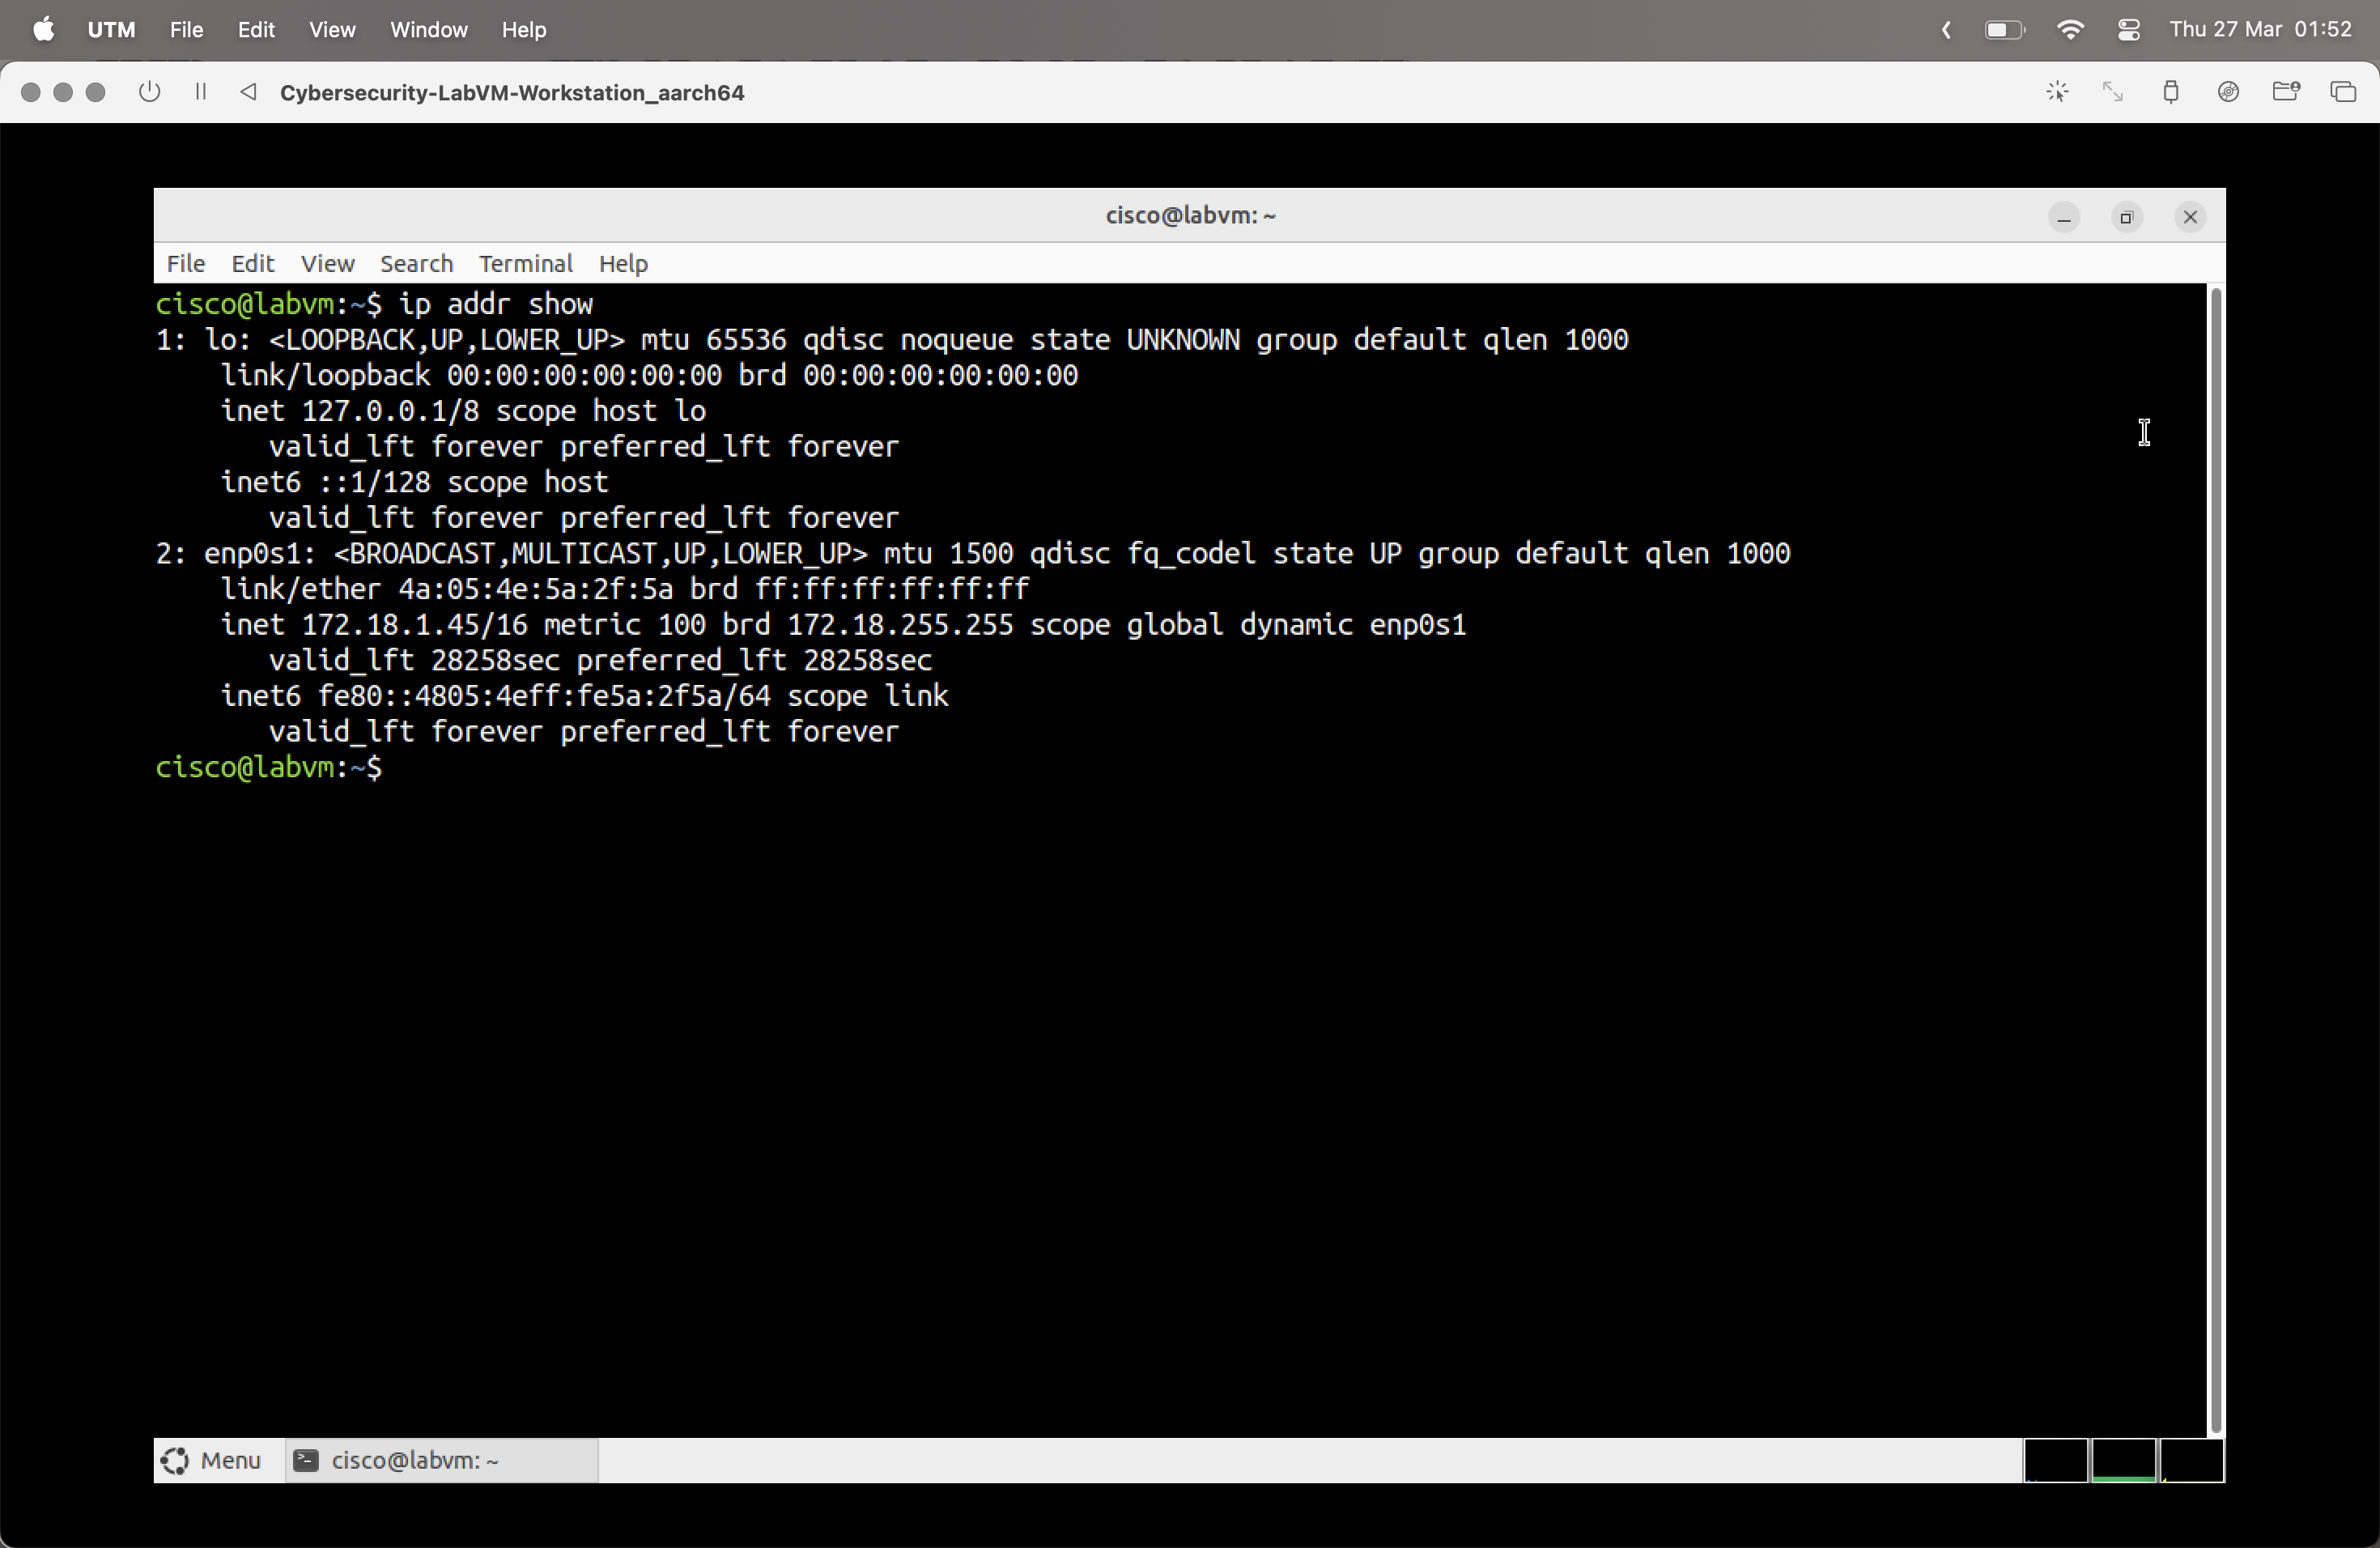
\includegraphics[width=0.8\textwidth]{lab1_ip_addr_show.png}
    \caption{Checking the ip of VM using command \textbf{ip addr show}}
\end{figure}

\subsubsection{Testing Web Server Access}
I confirmed that the Apache server was accessible from my host machine by navigating to the VM's IP address in a browser:

\begin{figure}[H]
    \centering
    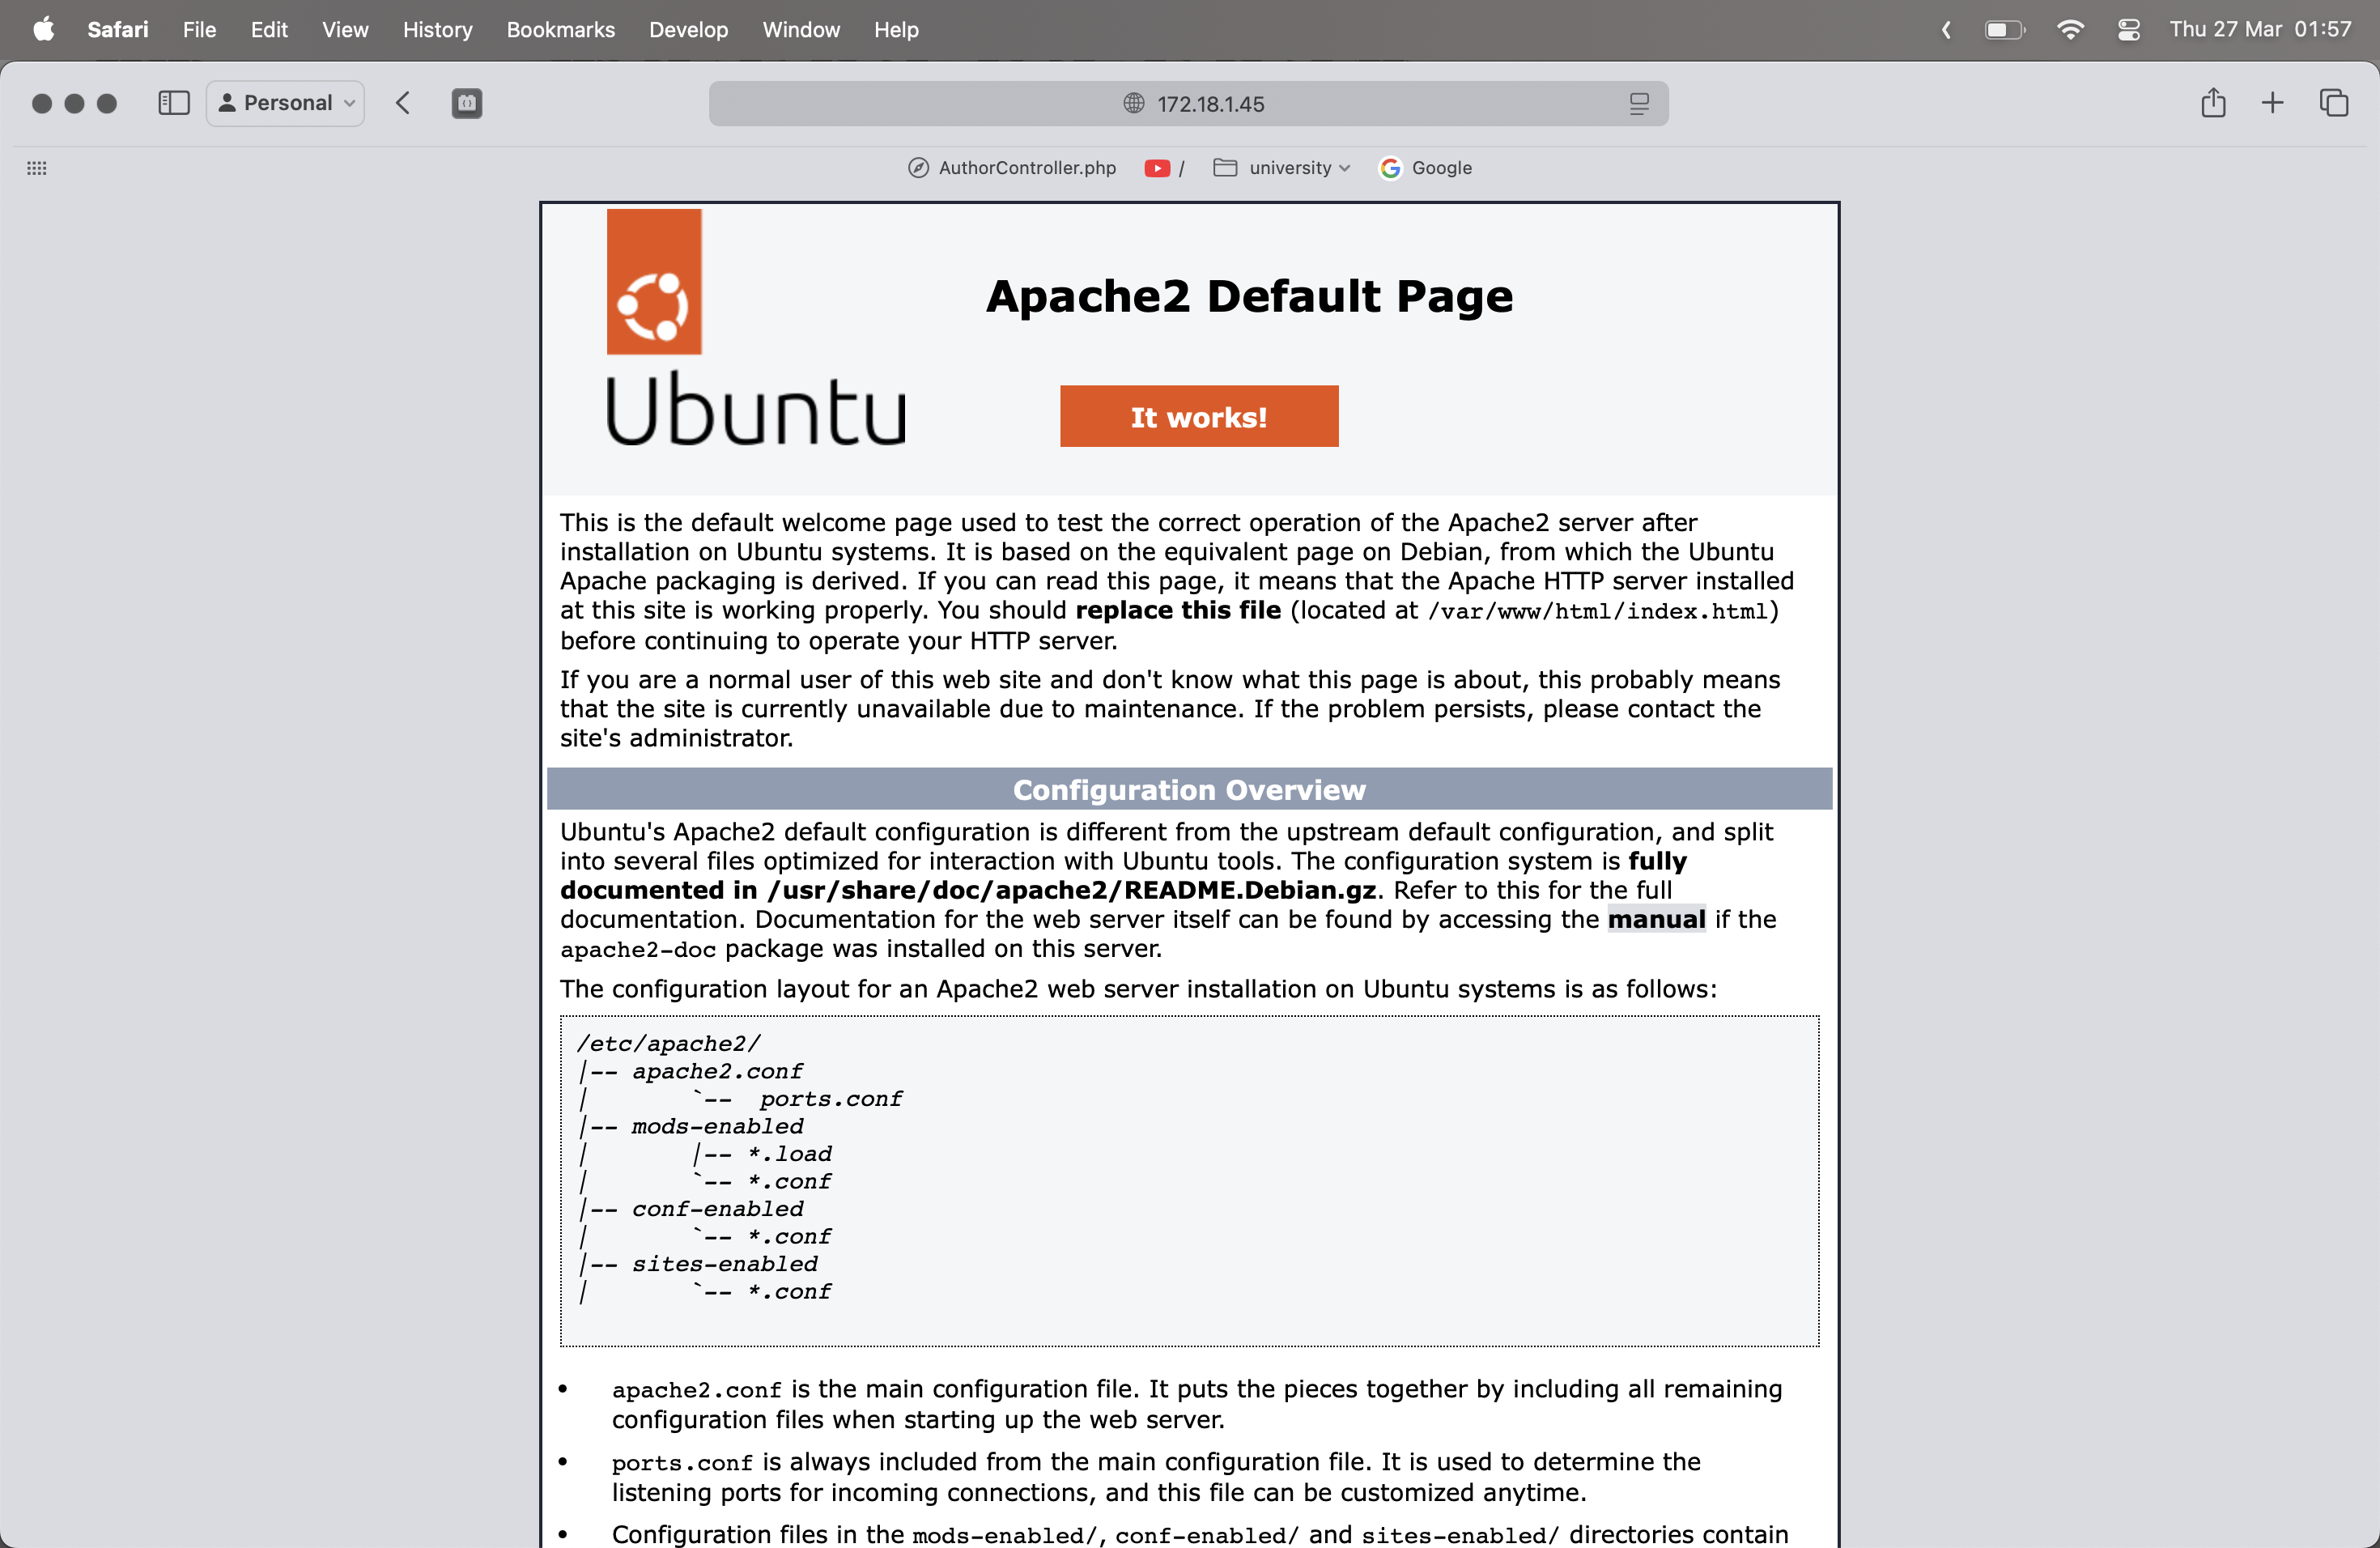
\includegraphics[width=0.8\textwidth]{lab1_apache_page.png}
    \caption{Default Apache page displayed in browser}
\end{figure}

\subsubsection{Configuring Firewall Rules}
I implemented the following iptables rules:

\begin{enumerate}
    \item First blocked HTTP traffic:
    \begin{lstlisting}
    sudo iptables -I INPUT 1 -p tcp --destination-port 80 -j DROP
    \end{lstlisting}
    
    \item Verified the block was effective by attempting to access the server again:
    \begin{figure}[H]
        \centering
        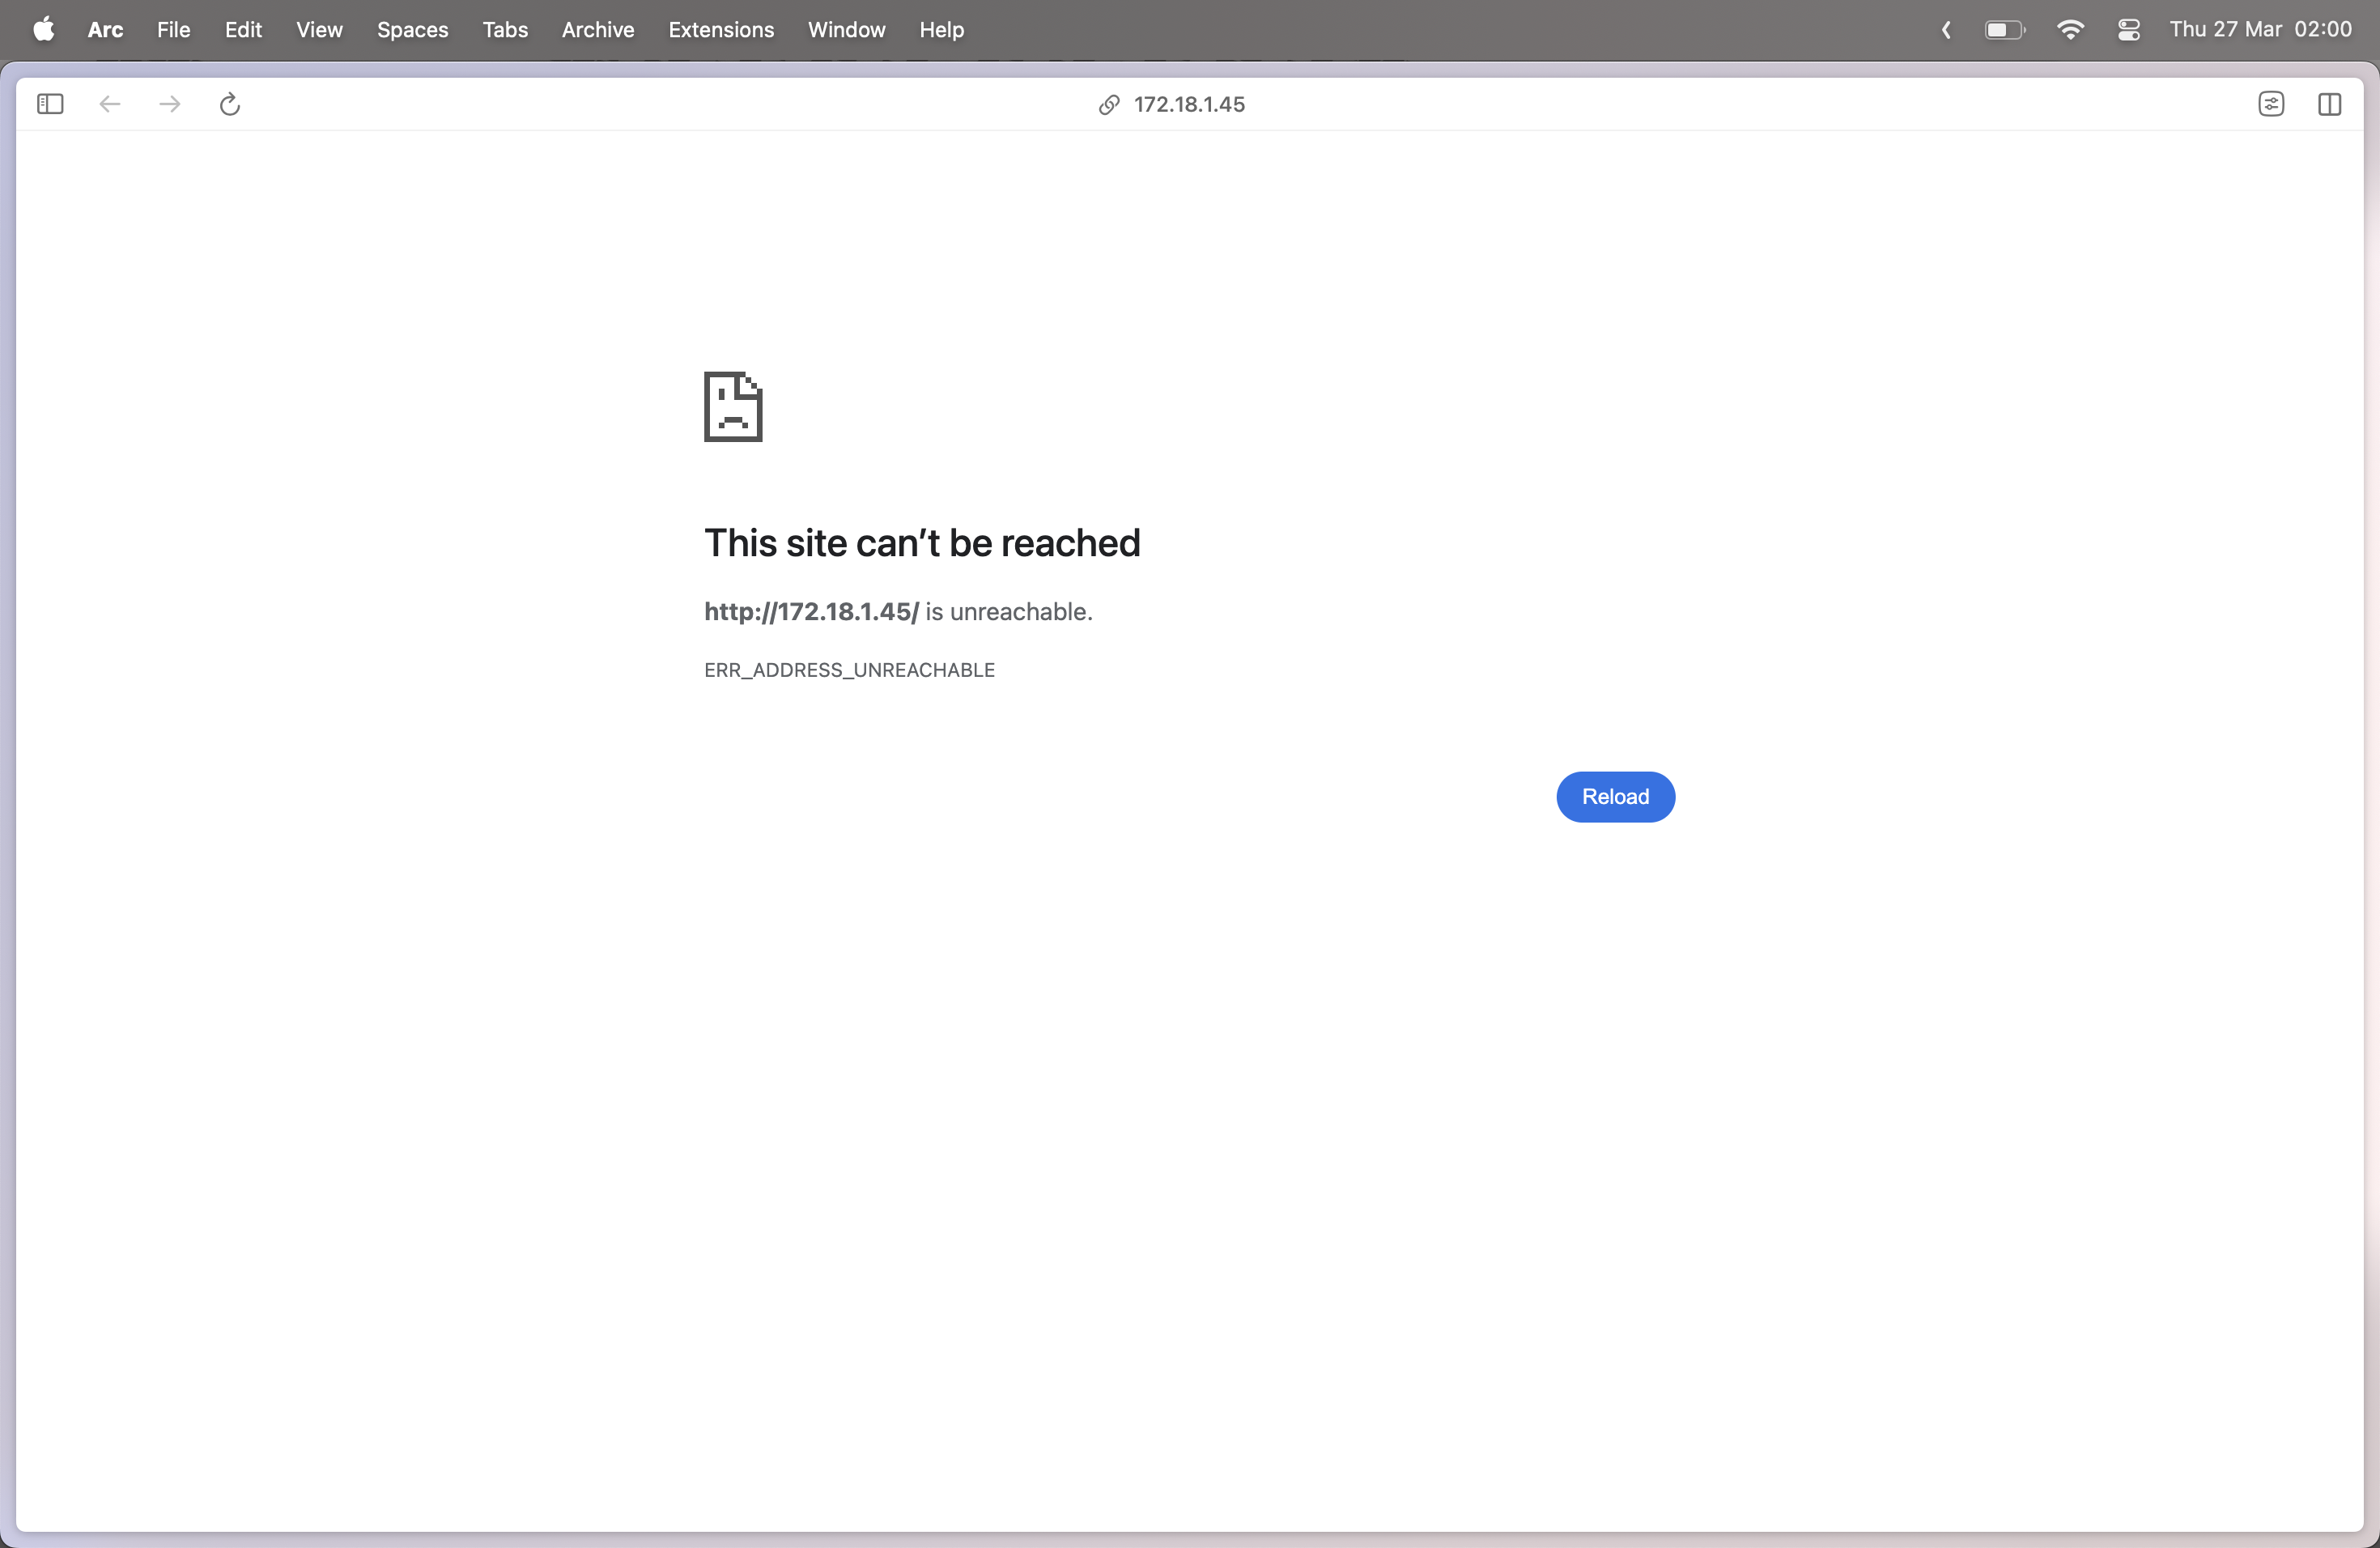
\includegraphics[width=0.8\textwidth]{lab1_connection_failed.png}
        \caption{Connection failed after blocking port 80}
    \end{figure}
    
    \item Re-enabled HTTP access:
    \begin{lstlisting}
    sudo iptables -I INPUT 1 -p tcp --destination-port 80 -j ACCEPT
    \end{lstlisting}
    
    \item Added logging to monitor traffic:
    \begin{lstlisting}
    sudo iptables -I INPUT 1 -j LOG
    \end{lstlisting}
\end{enumerate}

The final rule configuration looked like this:

\begin{figure}[H]
    \centering
    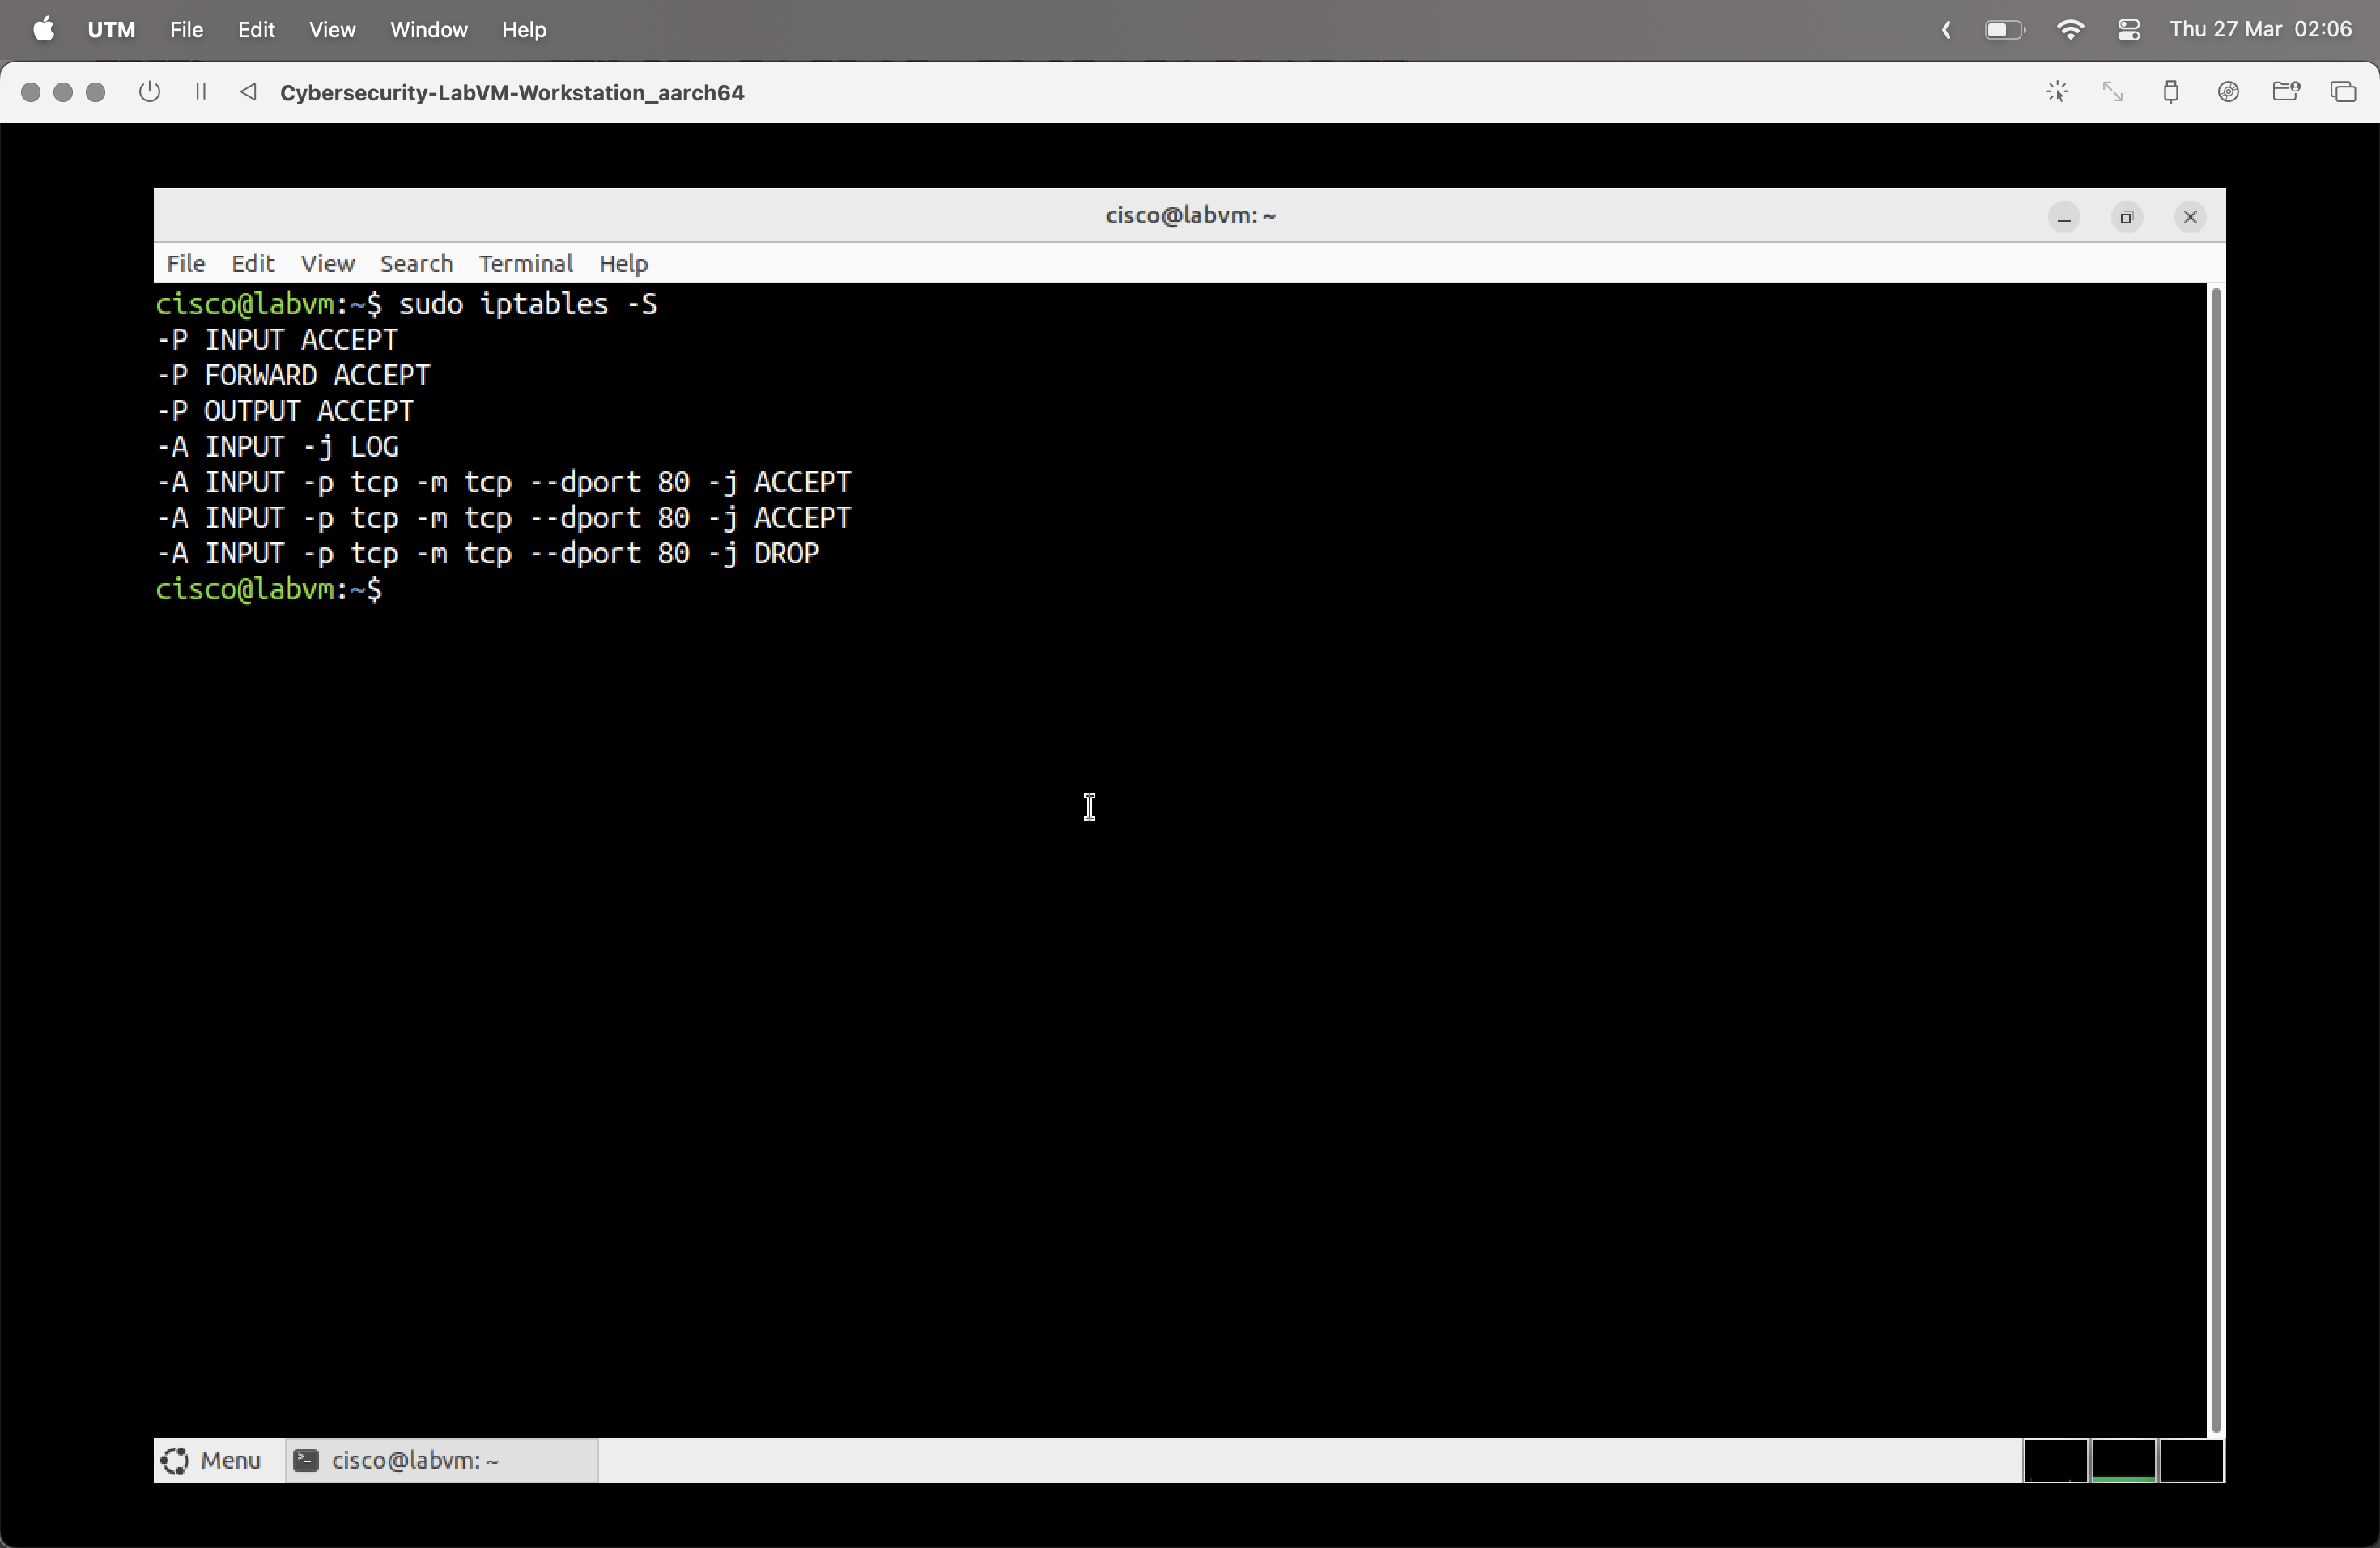
\includegraphics[width=0.8\textwidth]{lab1_iptables_rules.png}
    \caption{Final iptables rule configuration}
\end{figure}


\subsubsection{Analyzing Firewall Logs}
I examined the logs using the following command:
\begin{lstlisting}
sudo tail /var/log/kern.log | grep "80"
\end{lstlisting}

\begin{figure}[H]
    \centering
    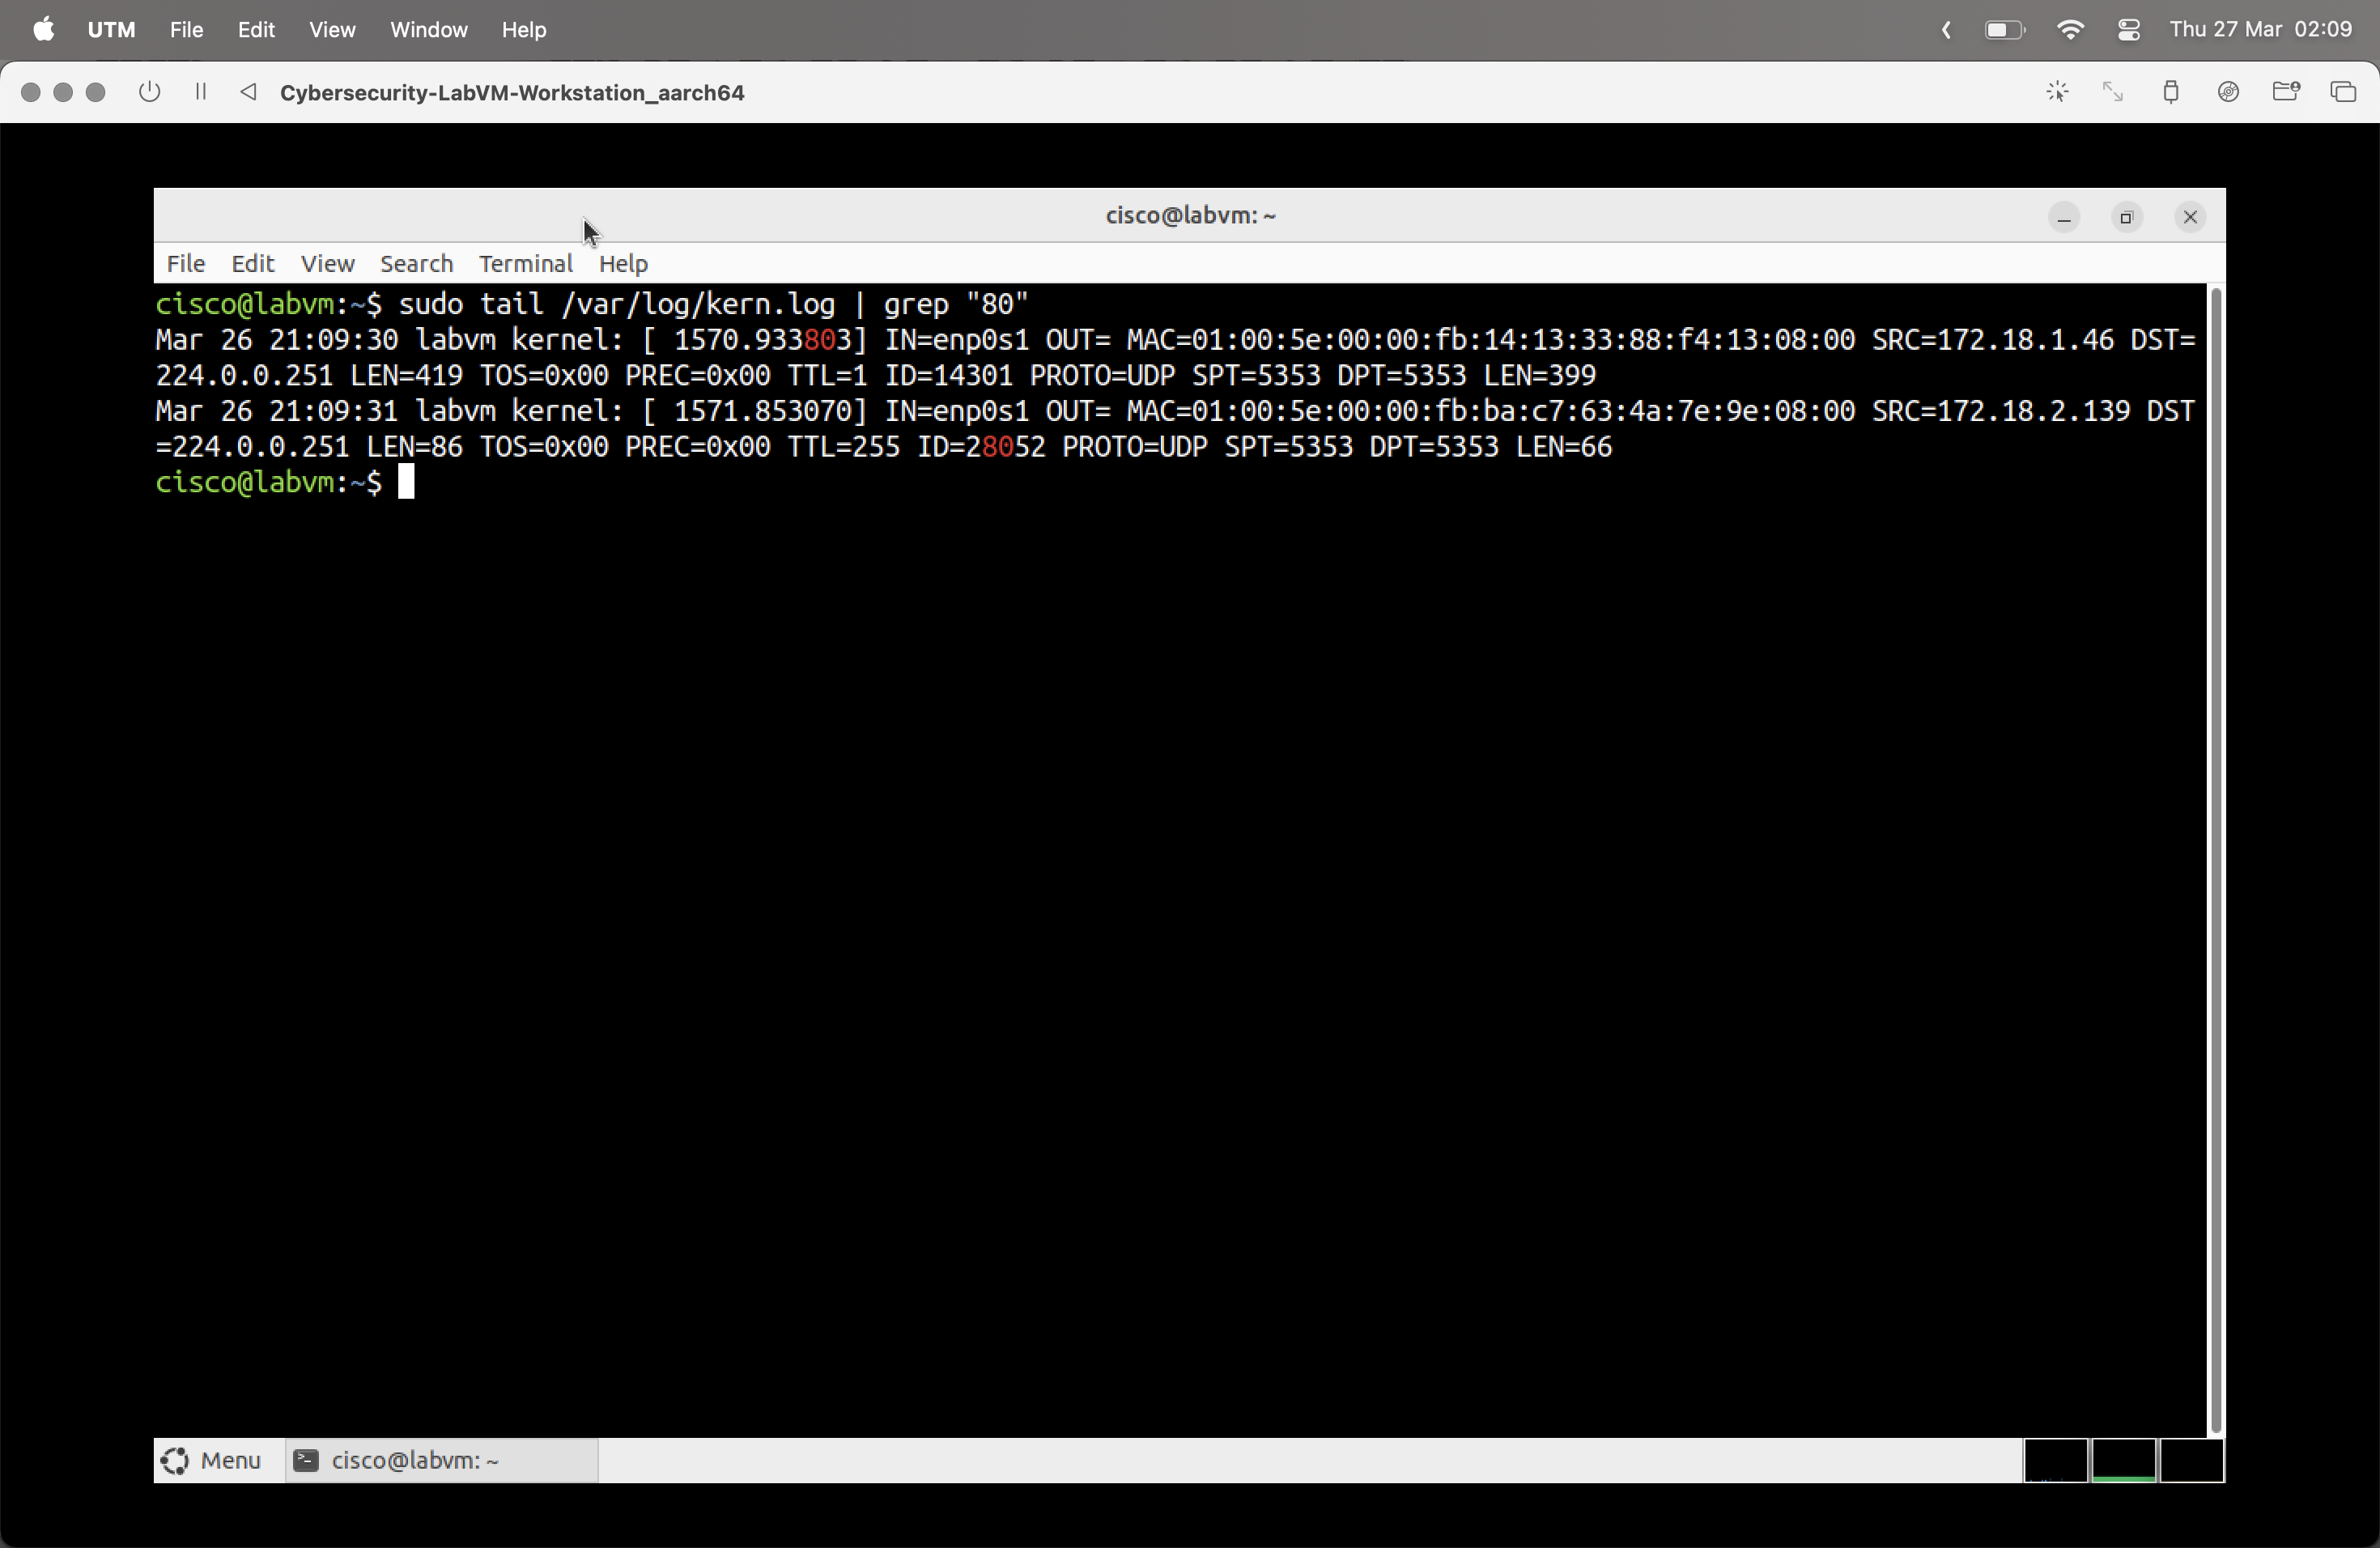
\includegraphics[width=0.8\textwidth]{lab1_firewall_logs.png}
    \caption{Firewall Logs}
\end{figure}

From the logs, I observed:

\begin{itemize}
    \item The source IP addresses attempting to connect to the server
    \item The packet types (SYN, ACK, etc.) being exchanged
    \item Connection attempts with their timestamps
    \item Request frequencies and patterns
\end{itemize}

\subsection{Lab 1 Conclusion}
Through this lab, I learned how to:
\begin{itemize}
    \item Configure Linux firewall rules using iptables
    \item Understand the relationship between firewall rules and network services
    \item Monitor and interpret network traffic using system logs
    \item Apply rule ordering to achieve desired network security policies
\end{itemize}

This exercise demonstrated how firewalls can be used to protect servers by controlling access to specific ports, and highlighted the importance of monitoring network traffic for security purposes.

\newpage
\section{Lab 2: Using a Port Scanner to Detect Open Ports}

\subsection{Objective}
The main objective of this lab was to use Nmap to scan for open ports on a system and analyze the security implications of these findings.

\subsection{TCP Port Scanning Results}

I ran a basic Nmap scan against localhost:

\begin{figure}[H]
    \centering
    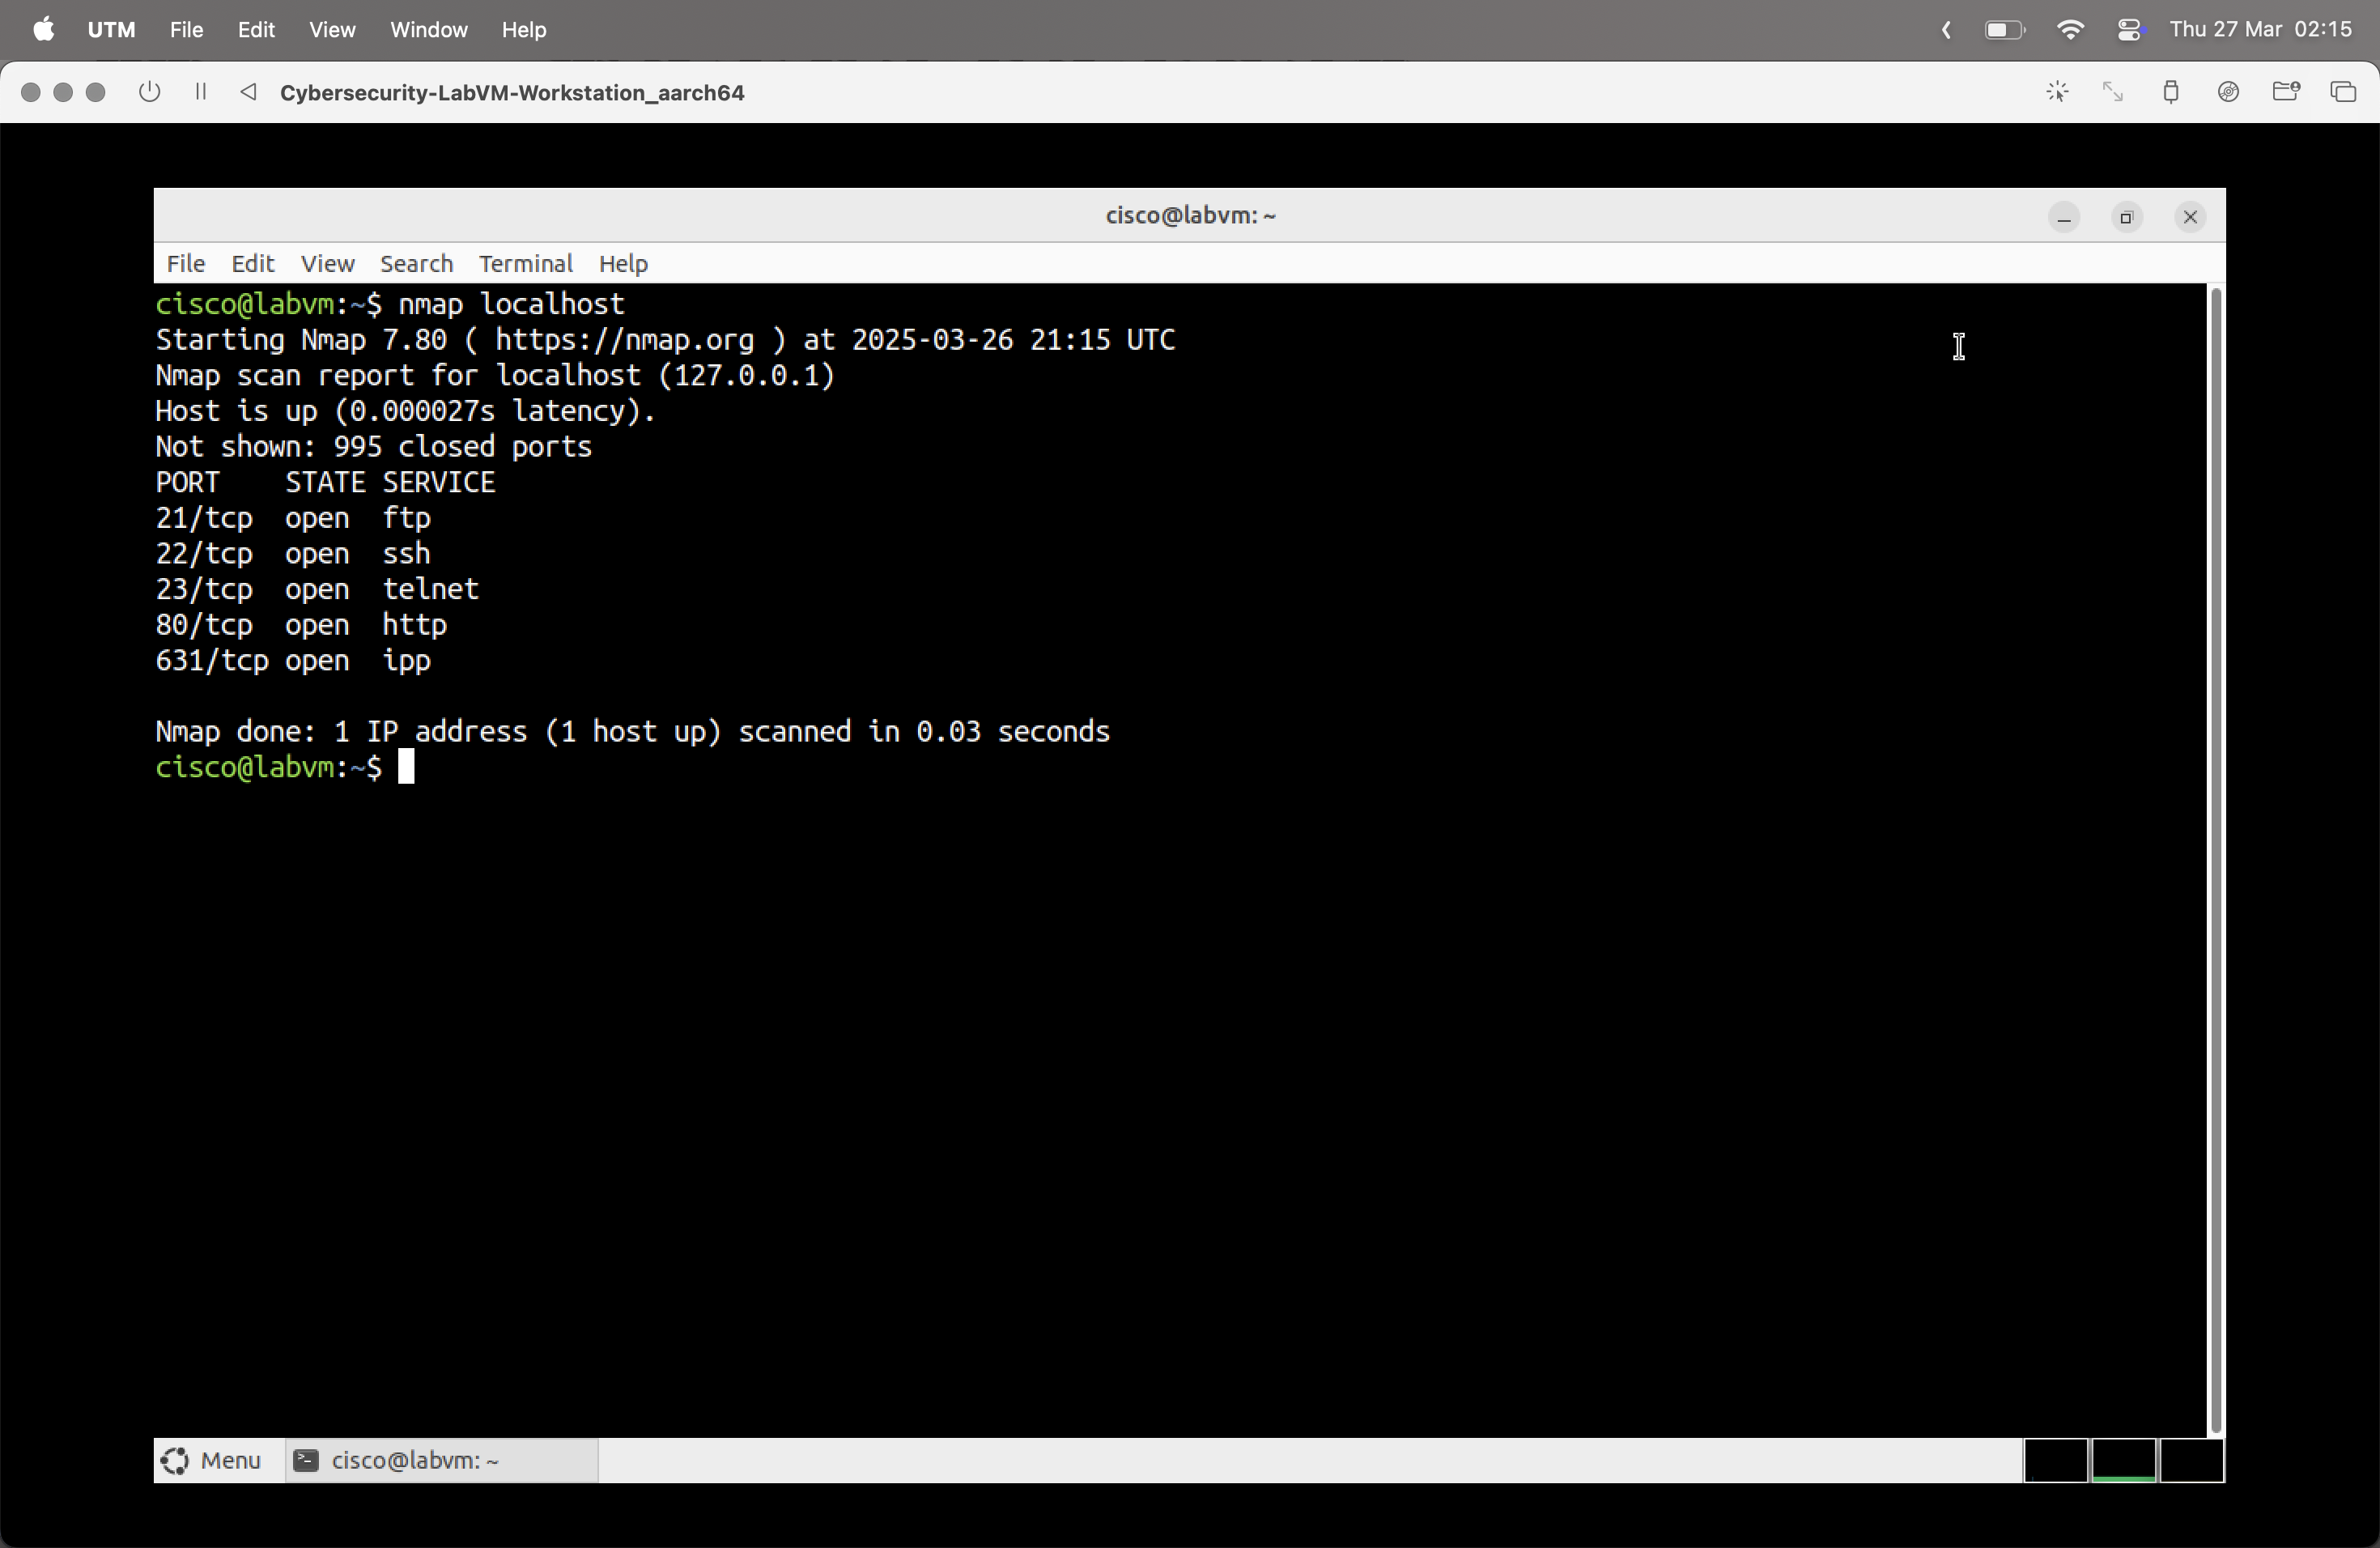
\includegraphics[width=0.8\textwidth]{lab2_nmap_basic.png}
    \caption{Basic Nmap scan results showing open TCP ports}
\end{figure}

\textbf{Open TCP Ports Found:}
\begin{itemize}
    \item Port 21 (ftp)
    \item Port 22 (SSH)
    \item Port 23 (Telnet)
    \item Port 80 (http)
    \item Port 631 (IPP)
\end{itemize}

\textbf{Service Analysis:}
\begin{itemize}
    \item \textbf{FTP (Port 21)} - File Transfer Protocol used for transferring files between systems. By default, it transmits credentials and data in plaintext, making it insecure without encryption (FTPS or SFTP).
    
    \item \textbf{SSH (Port 22)} - Secure Shell provides encrypted remote access and administration, replacing insecure alternatives like Telnet.
    
    \item \textbf{Telnet (Port 23)} - An unencrypted protocol for remote terminal access. It sends all data, including passwords, in plaintext, making it highly vulnerable.
    
    \item \textbf{HTTP (Port 80)} - Hypertext Transfer Protocol used for web communication. Without HTTPS (TLS encryption), traffic can be intercepted or modified.
    
    \item \textbf{IPP (Port 631)} - Internet Printing Protocol used by CUPS (Common Unix Printing System) for network printing services.
\end{itemize}

\textbf{Vulnerability Analysis:}
\begin{itemize}
    \item \textbf{FTP}: Susceptible to brute-force attacks and MITM (Man-in-the-Middle) attacks. Unencrypted data transmission exposes credentials and files. Anonymous access misconfigurations can lead to data exposure.
    
    \item \textbf{SSH}: While secure, it is a common target for brute-force attacks if weak passwords are used. Older versions may contain vulnerabilities like CVE-2021-41617.
    
    \item \textbf{Telnet}: Completely insecure due to plaintext data transmission. Attackers can intercept credentials using packet sniffing. It should be replaced with SSH.
    
    \item \textbf{HTTP}: Vulnerable to MITM attacks if no SSL/TLS is used. Prone to SQL injection, Cross-Site Scripting (XSS), and other web-based exploits.
    
    \item \textbf{IPP}: The CUPS service on port 631 has had multiple reported vulnerabilities, including privilege escalation, denial-of-service (DoS) attacks, and unauthorized access to print jobs.
\end{itemize}

\subsection{UDP Port Scanning Results}

I scanned for open UDP ports using sudo privileges:

\begin{figure}[H]
    \centering
    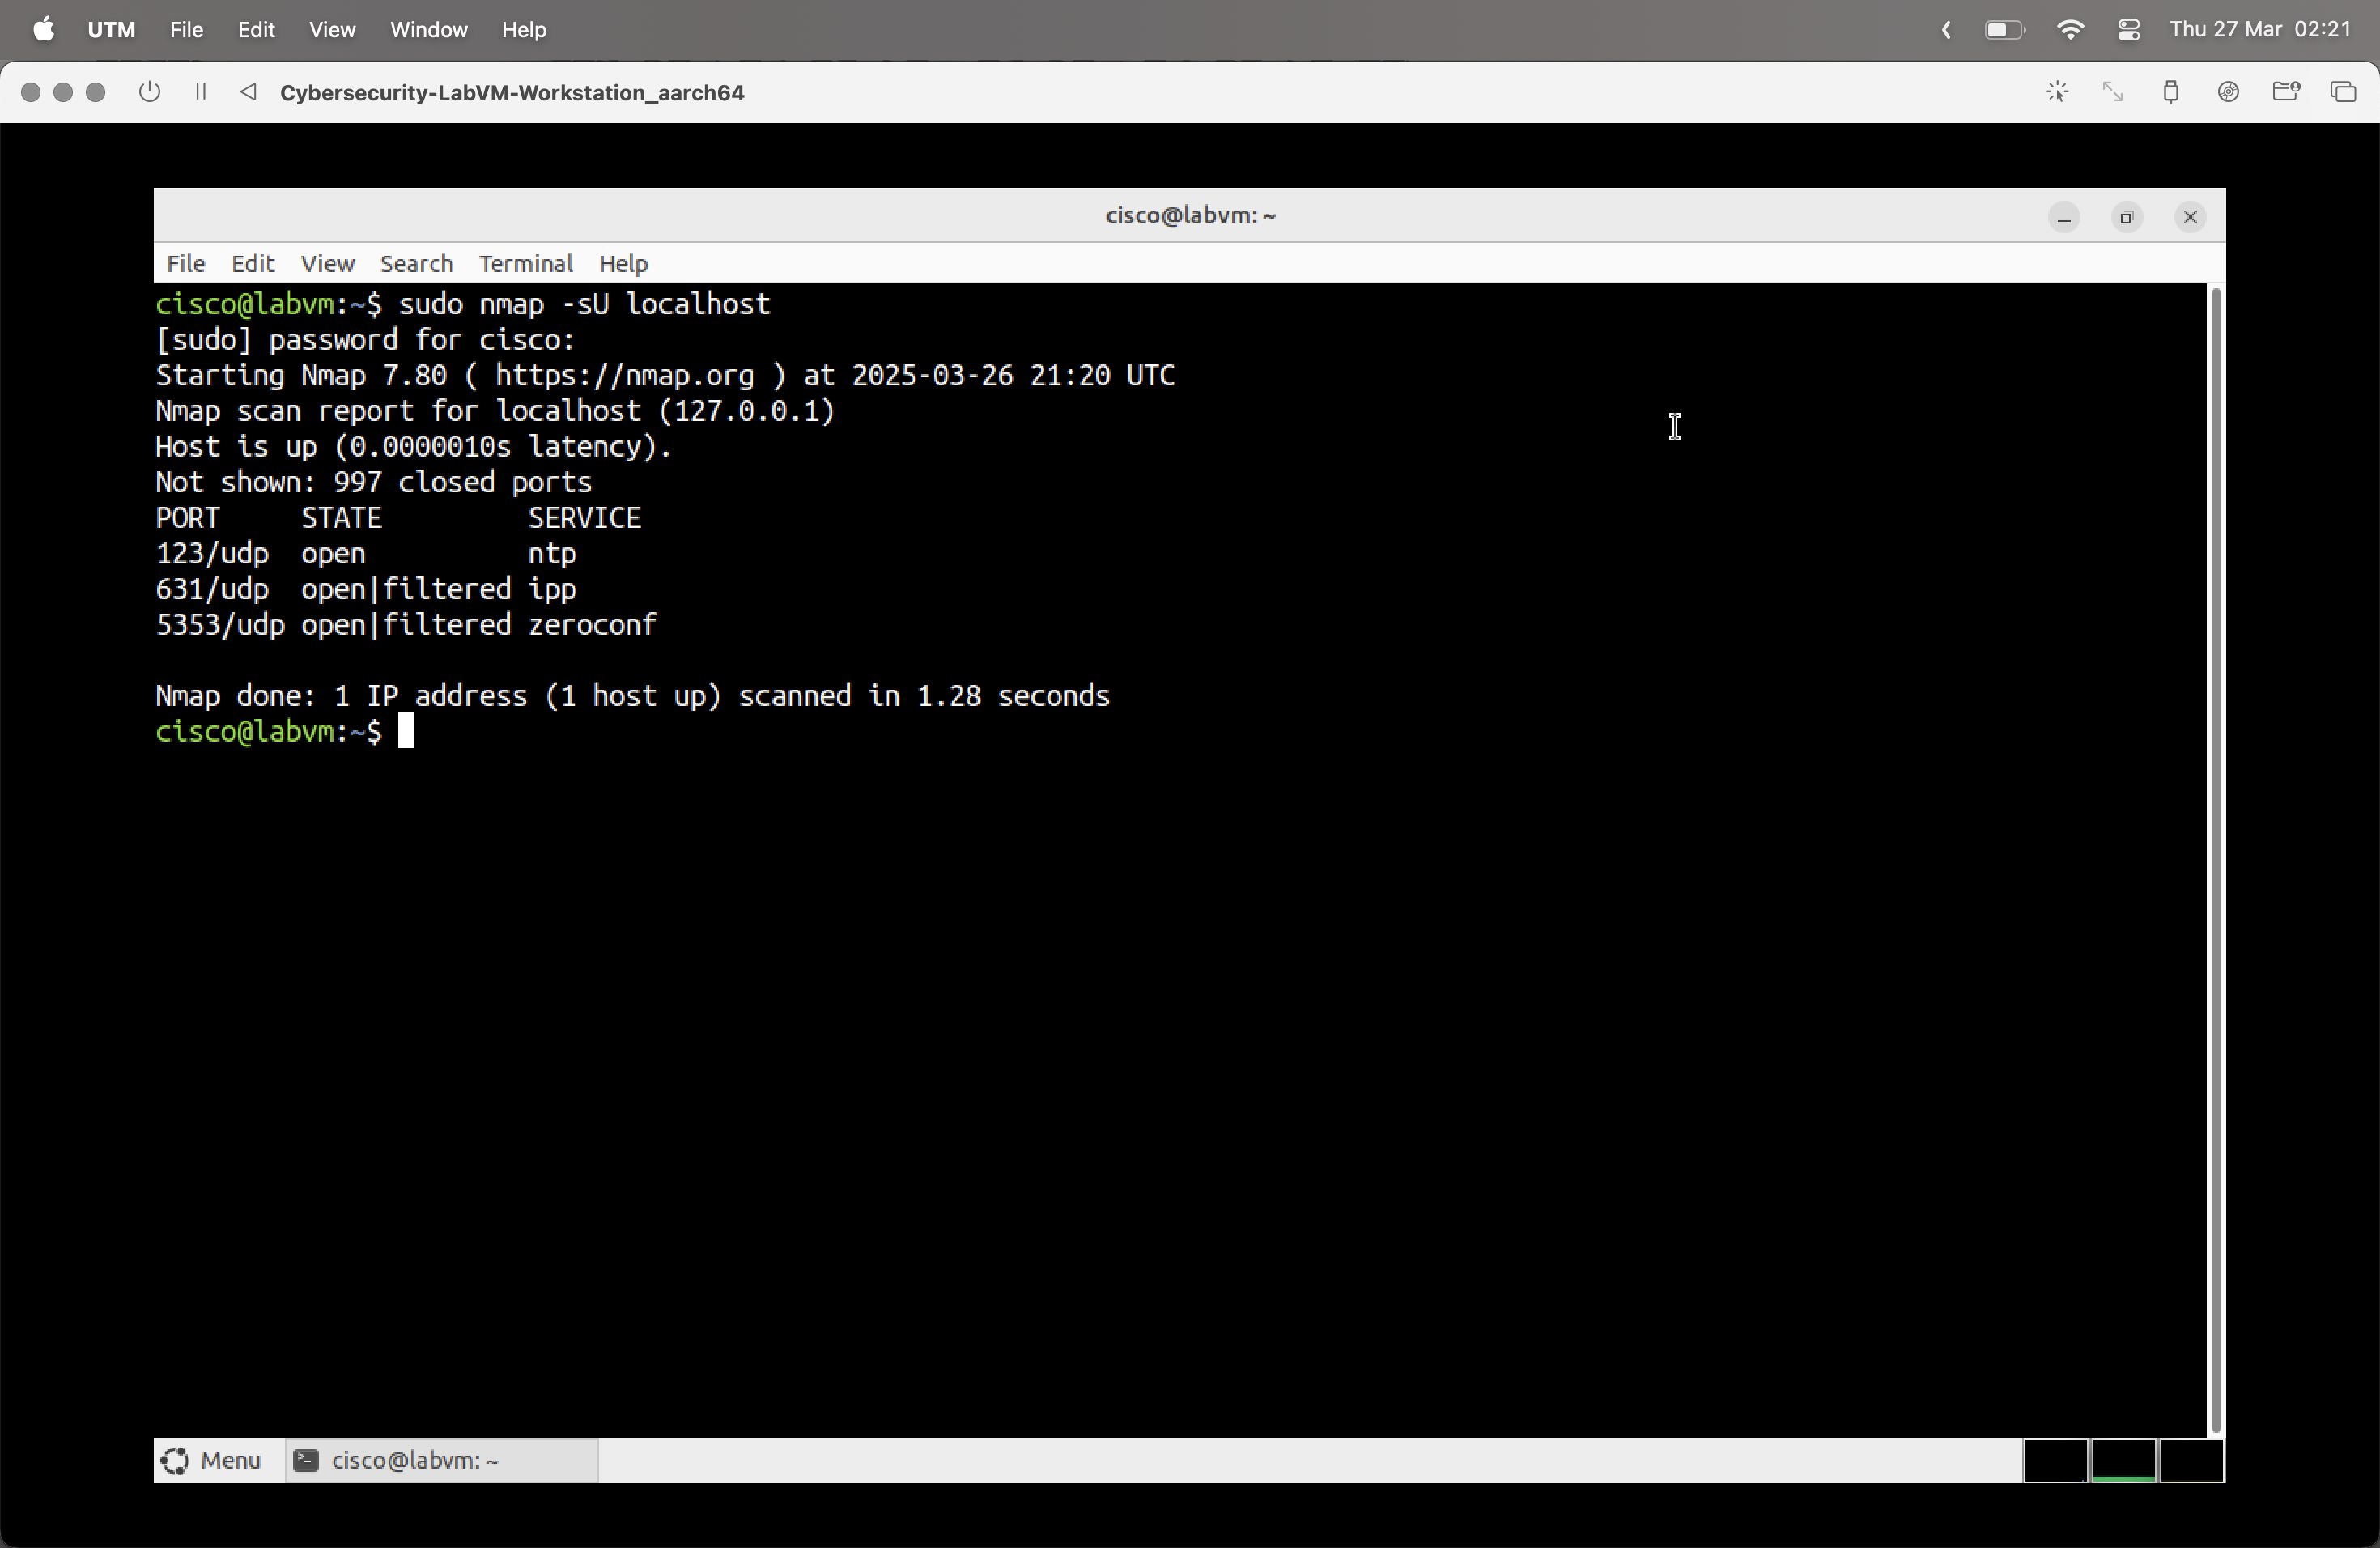
\includegraphics[width=0.8\textwidth]{lab2_nmap_udp.png}
    \caption{Nmap UDP scan results}
\end{figure}

\newpage

\textbf{Open UDP Ports Found:}
\begin{itemize}
    \item Port 123 (NTP)
    \item Port 631 (IPP)
    \item Port 5353 (Zeroconf/mDNS)
\end{itemize}

\textbf{Service Analysis:}
\begin{itemize}
    \item \textbf{NTP (Port 123)} - Network Time Protocol is used to synchronize system clocks across a network. It ensures accurate timekeeping for security protocols and system logs.
    
    \item \textbf{IPP (Port 631)} - Internet Printing Protocol is used by CUPS (Common Unix Printing System) for network printing and printer management.
    
    \item \textbf{Zeroconf/mDNS (Port 5353)} - Multicast DNS (mDNS) is used for service discovery on local networks, allowing devices to find each other without a central DNS server.
\end{itemize}

\textbf{Vulnerability Analysis:}
\begin{itemize}
    \item \textbf{NTP}: Vulnerable to amplification attacks, where an attacker spoofs the victim's IP address and floods it with large responses (NTP reflection attack). Older NTP versions may also be susceptible to DoS and time manipulation attacks.
    
    \item \textbf{IPP}: The CUPS service has had various security flaws, including privilege escalation and remote code execution vulnerabilities (e.g., CVE-2023-4504). Misconfigured printers may allow unauthorized access to print jobs.
    
    \item \textbf{Zeroconf/mDNS}: Vulnerable to information leakage and MITM (Man-in-the-Middle) attacks. Attackers can exploit mDNS to enumerate network services and potentially manipulate responses for phishing or network attacks.
\end{itemize}

\subsection{Service Version Detection}

I performed a service version scan to get more detailed information:

\begin{figure}[H]
    \centering
    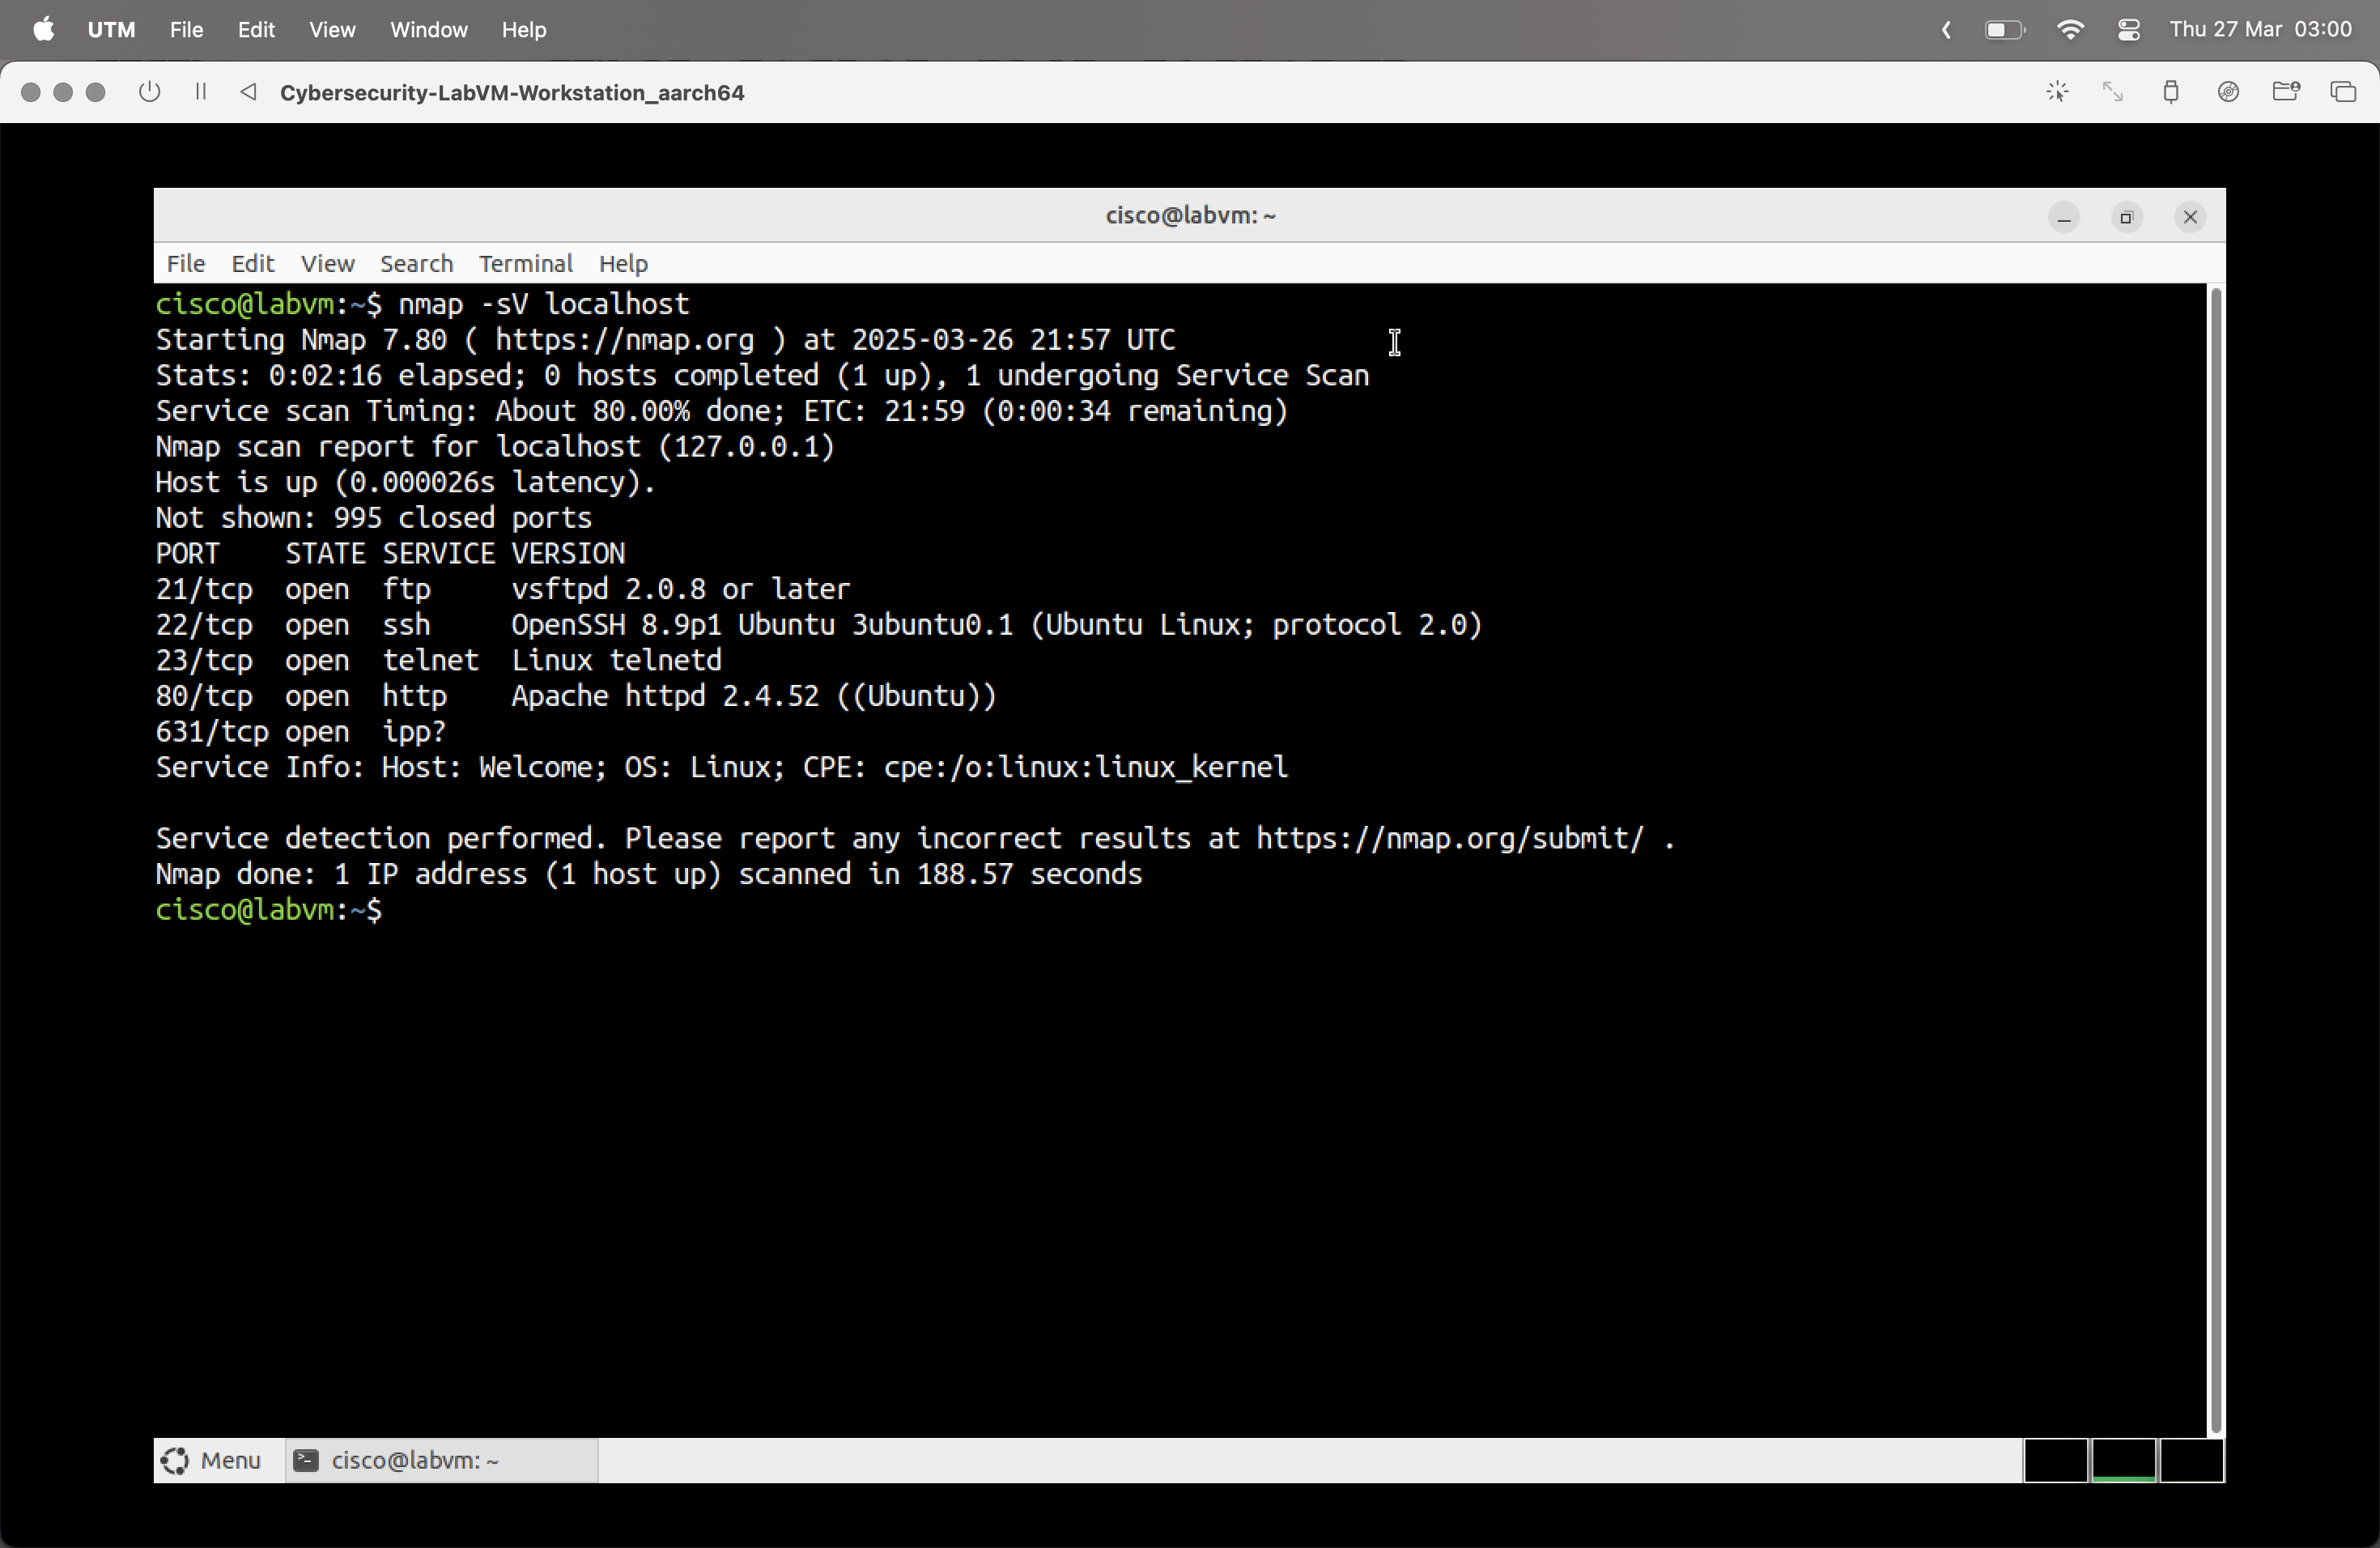
\includegraphics[width=0.8\textwidth]{lab2_nmap_version.png}
    \caption{Nmap service version detection results}
\end{figure}

This scan revealed specific software versions:
\begin{itemize}
    \item FTP: vsftpd 2.0.8 or later
    \item SSH: OpenSSH 8.9p1 Ubuntu 3ubuntu0.1
    \item Telnet: Linux telnetd
    \item HTTP: Apache httpd 2.4.52
    \item IPP: ?
\end{itemize}

These specific versions are important for vulnerability assessment, as each version may have particular known exploits.

\subsection{SSH Key Information}

Using the aggressive scanning mode, I obtained SSH host keys:

\begin{figure}[H]
    \centering
    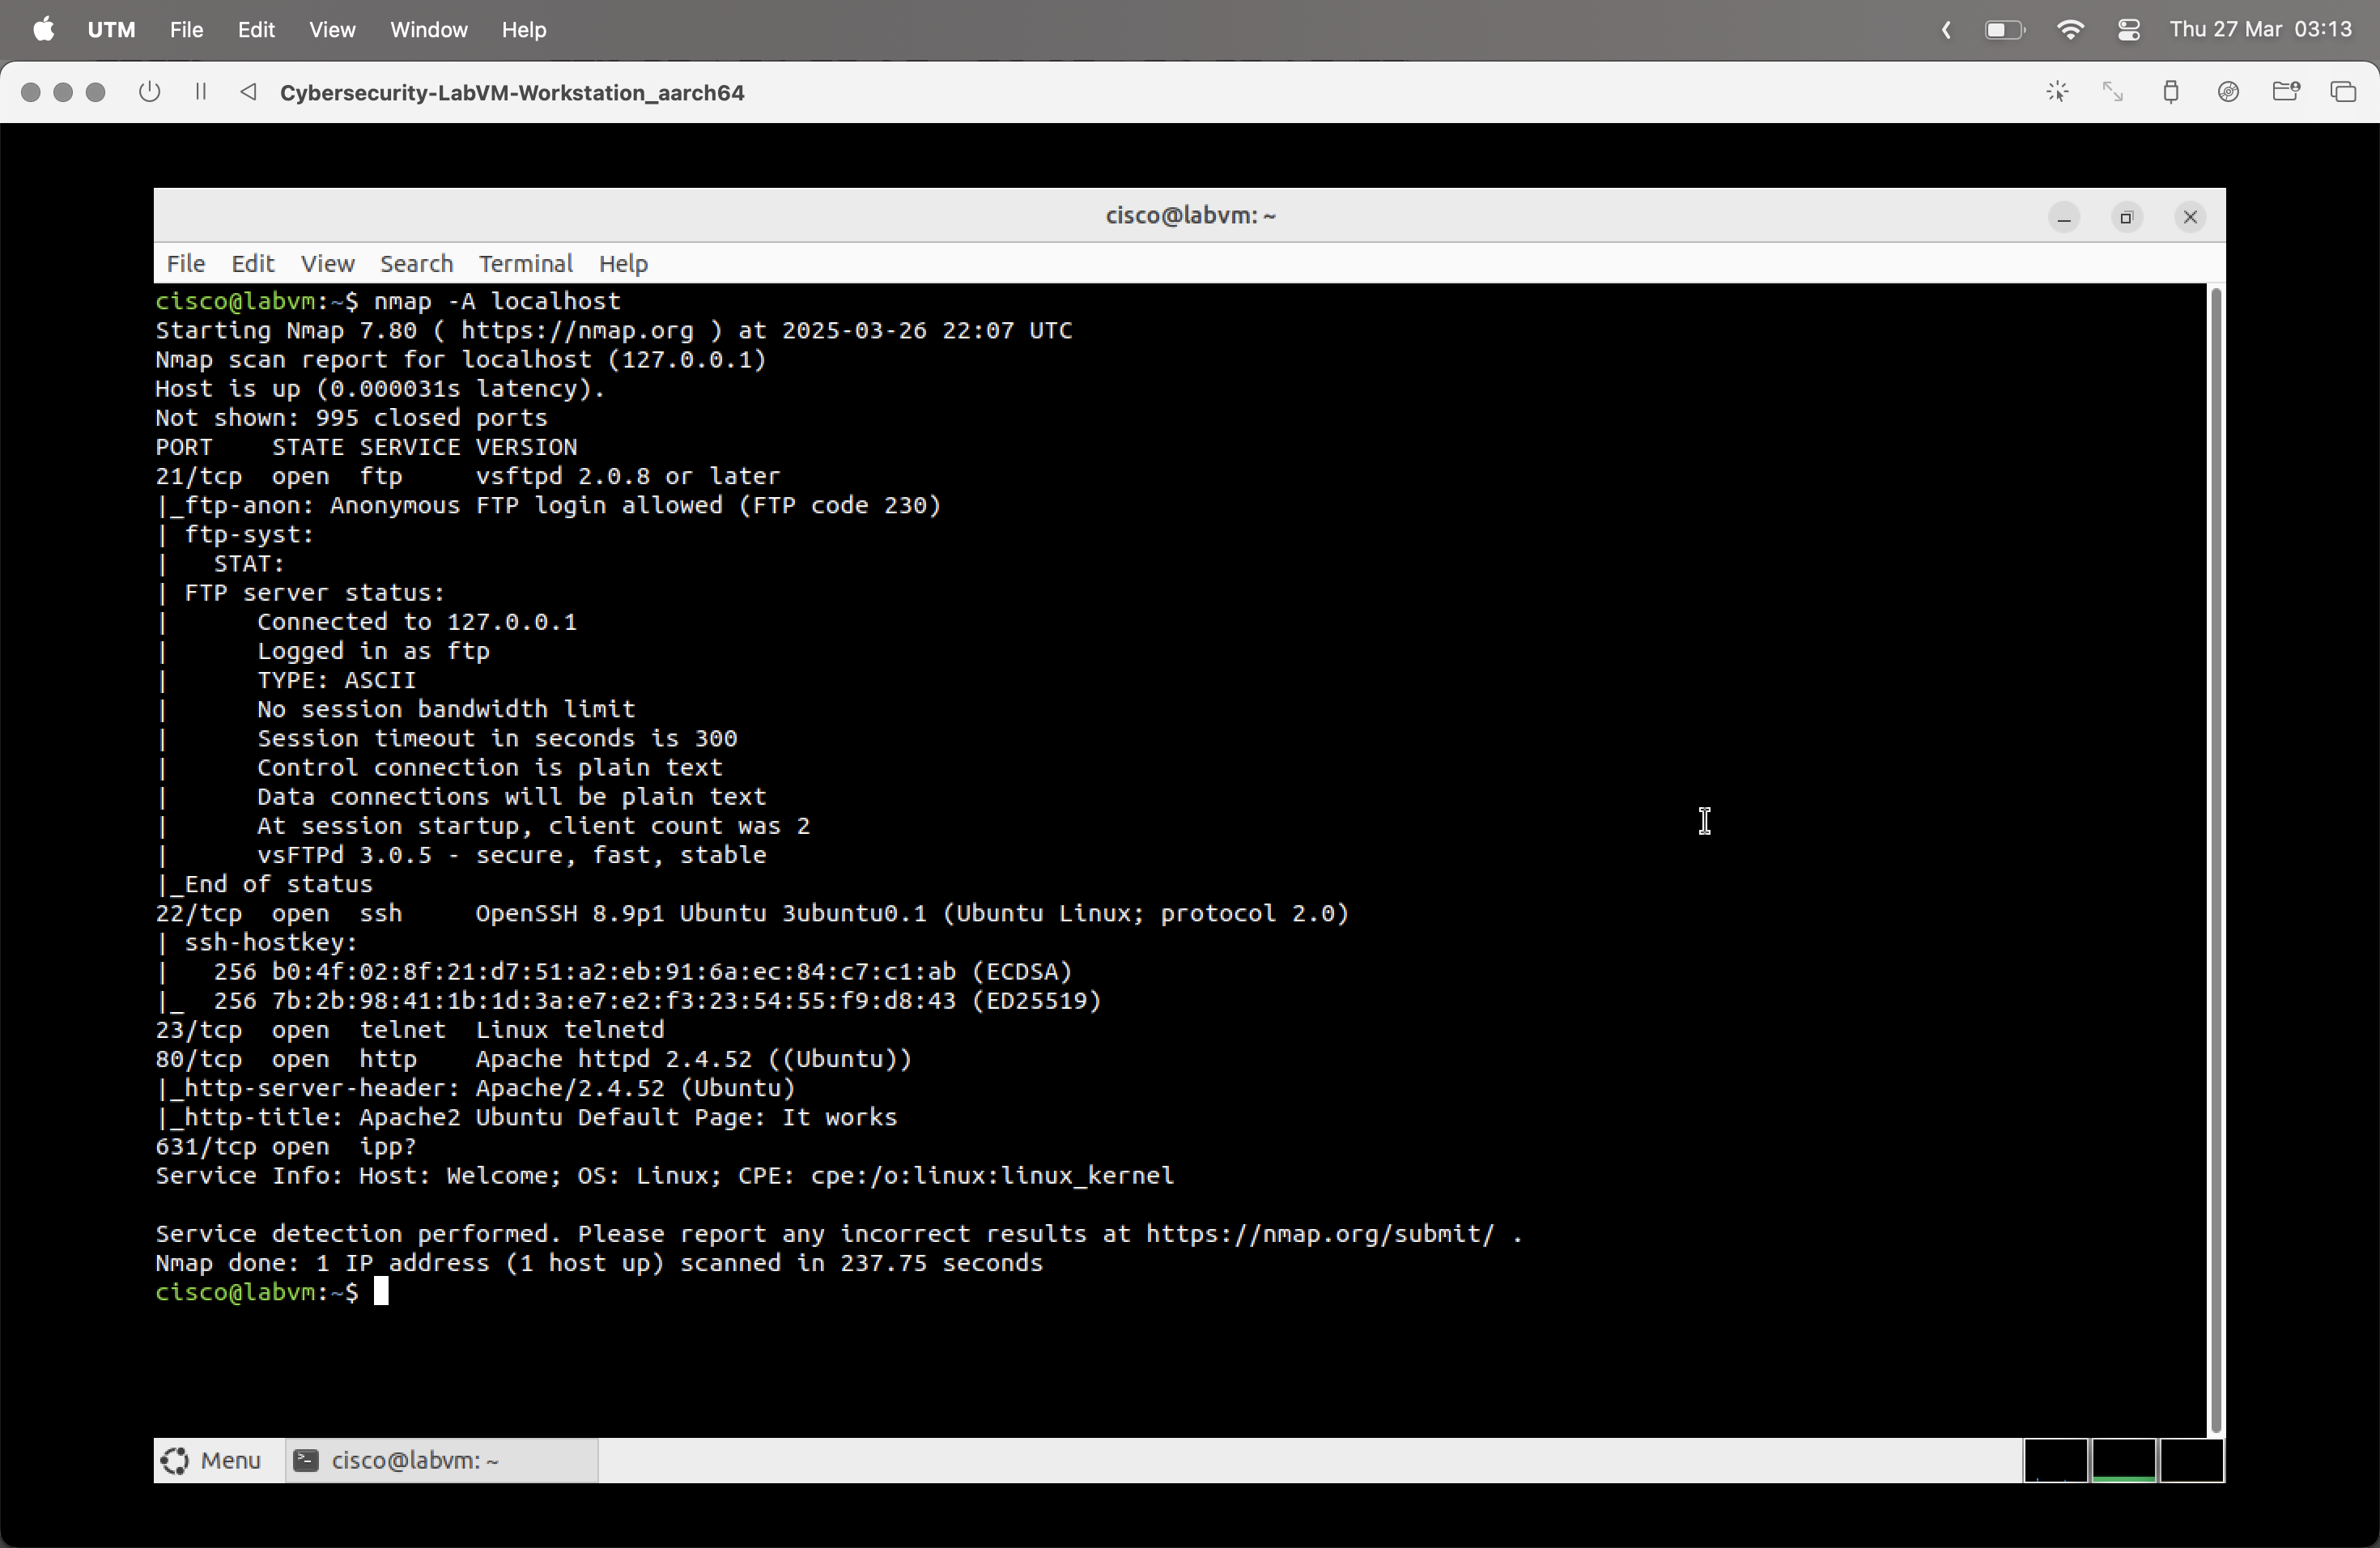
\includegraphics[width=0.8\textwidth]{lab2_nmap_aggressive.png}
    \caption{Nmap aggressive scan showing SSH host keys}
\end{figure}
 
\textbf{Captured SSH Host Keys:}
\begin{itemize}
    \item ECDSA (256-bit): \texttt{b0:4f:02:8f:21:d7:51:a2:eb:91:6a:ec:84:c7:c1:ab}
    \item ED25519 (256-bit): \texttt{7b:2b:98:41:1b:1d:3a:e7:e2:f3:23:54:55:f9:d8:43}
\end{itemize}

\textbf{How an Attacker Could Use This Information:}
\begin{itemize}
    \item Identify the system by its SSH fingerprint
    \item Detect if the server has been replaced (if the fingerprint changes)
    \item Perform SSH MITM attacks if hostkey verification is disabled
\end{itemize}

\textbf{Mitigation Strategies:}
\begin{itemize}
    \item Disable unnecessary SSH key types (like DSA)
    \item Use SSH key rotation policies
    \item Implement firewall rules to limit SSH access to trusted IP addresses
    \item Use key-based authentication instead of passwords
    \item Configure SSH to use stronger ciphers and MAC algorithms
\end{itemize}

\newpage

\subsection{Lab 2 Conclusion}
This port scanning exercise revealed several potential security issues:
\begin{itemize}
    \item The presence of Telnet (port 23) poses a significant security risk
    \item Multiple services (SSH, IPP, Zeroconf) provide potential attack vectors
    \item Detailed system information is discoverable through simple scanning techniques
\end{itemize}
To improve security, I would recommend:
\begin{itemize}
    \item Disabling Telnet entirely and using SSH exclusively
    \item Restricting access to necessary ports only
    \item Implementing proper authentication mechanisms
    \item Keeping all services updated to patch known vulnerabilities
    \item Configuring the firewall to limit access to these services
\end{itemize}


\newpage
\section{Lab 3: Hashing Things Out}

\subsection{Part 1: Hashing a Text File with OpenSSL}

In this part of the lab, I explored hash functions by creating and comparing hashes of text files.

\subsubsection{Initial Text File Hashing}

I first examined the contents of the text file:

\begin{figure}[H]
    \centering
    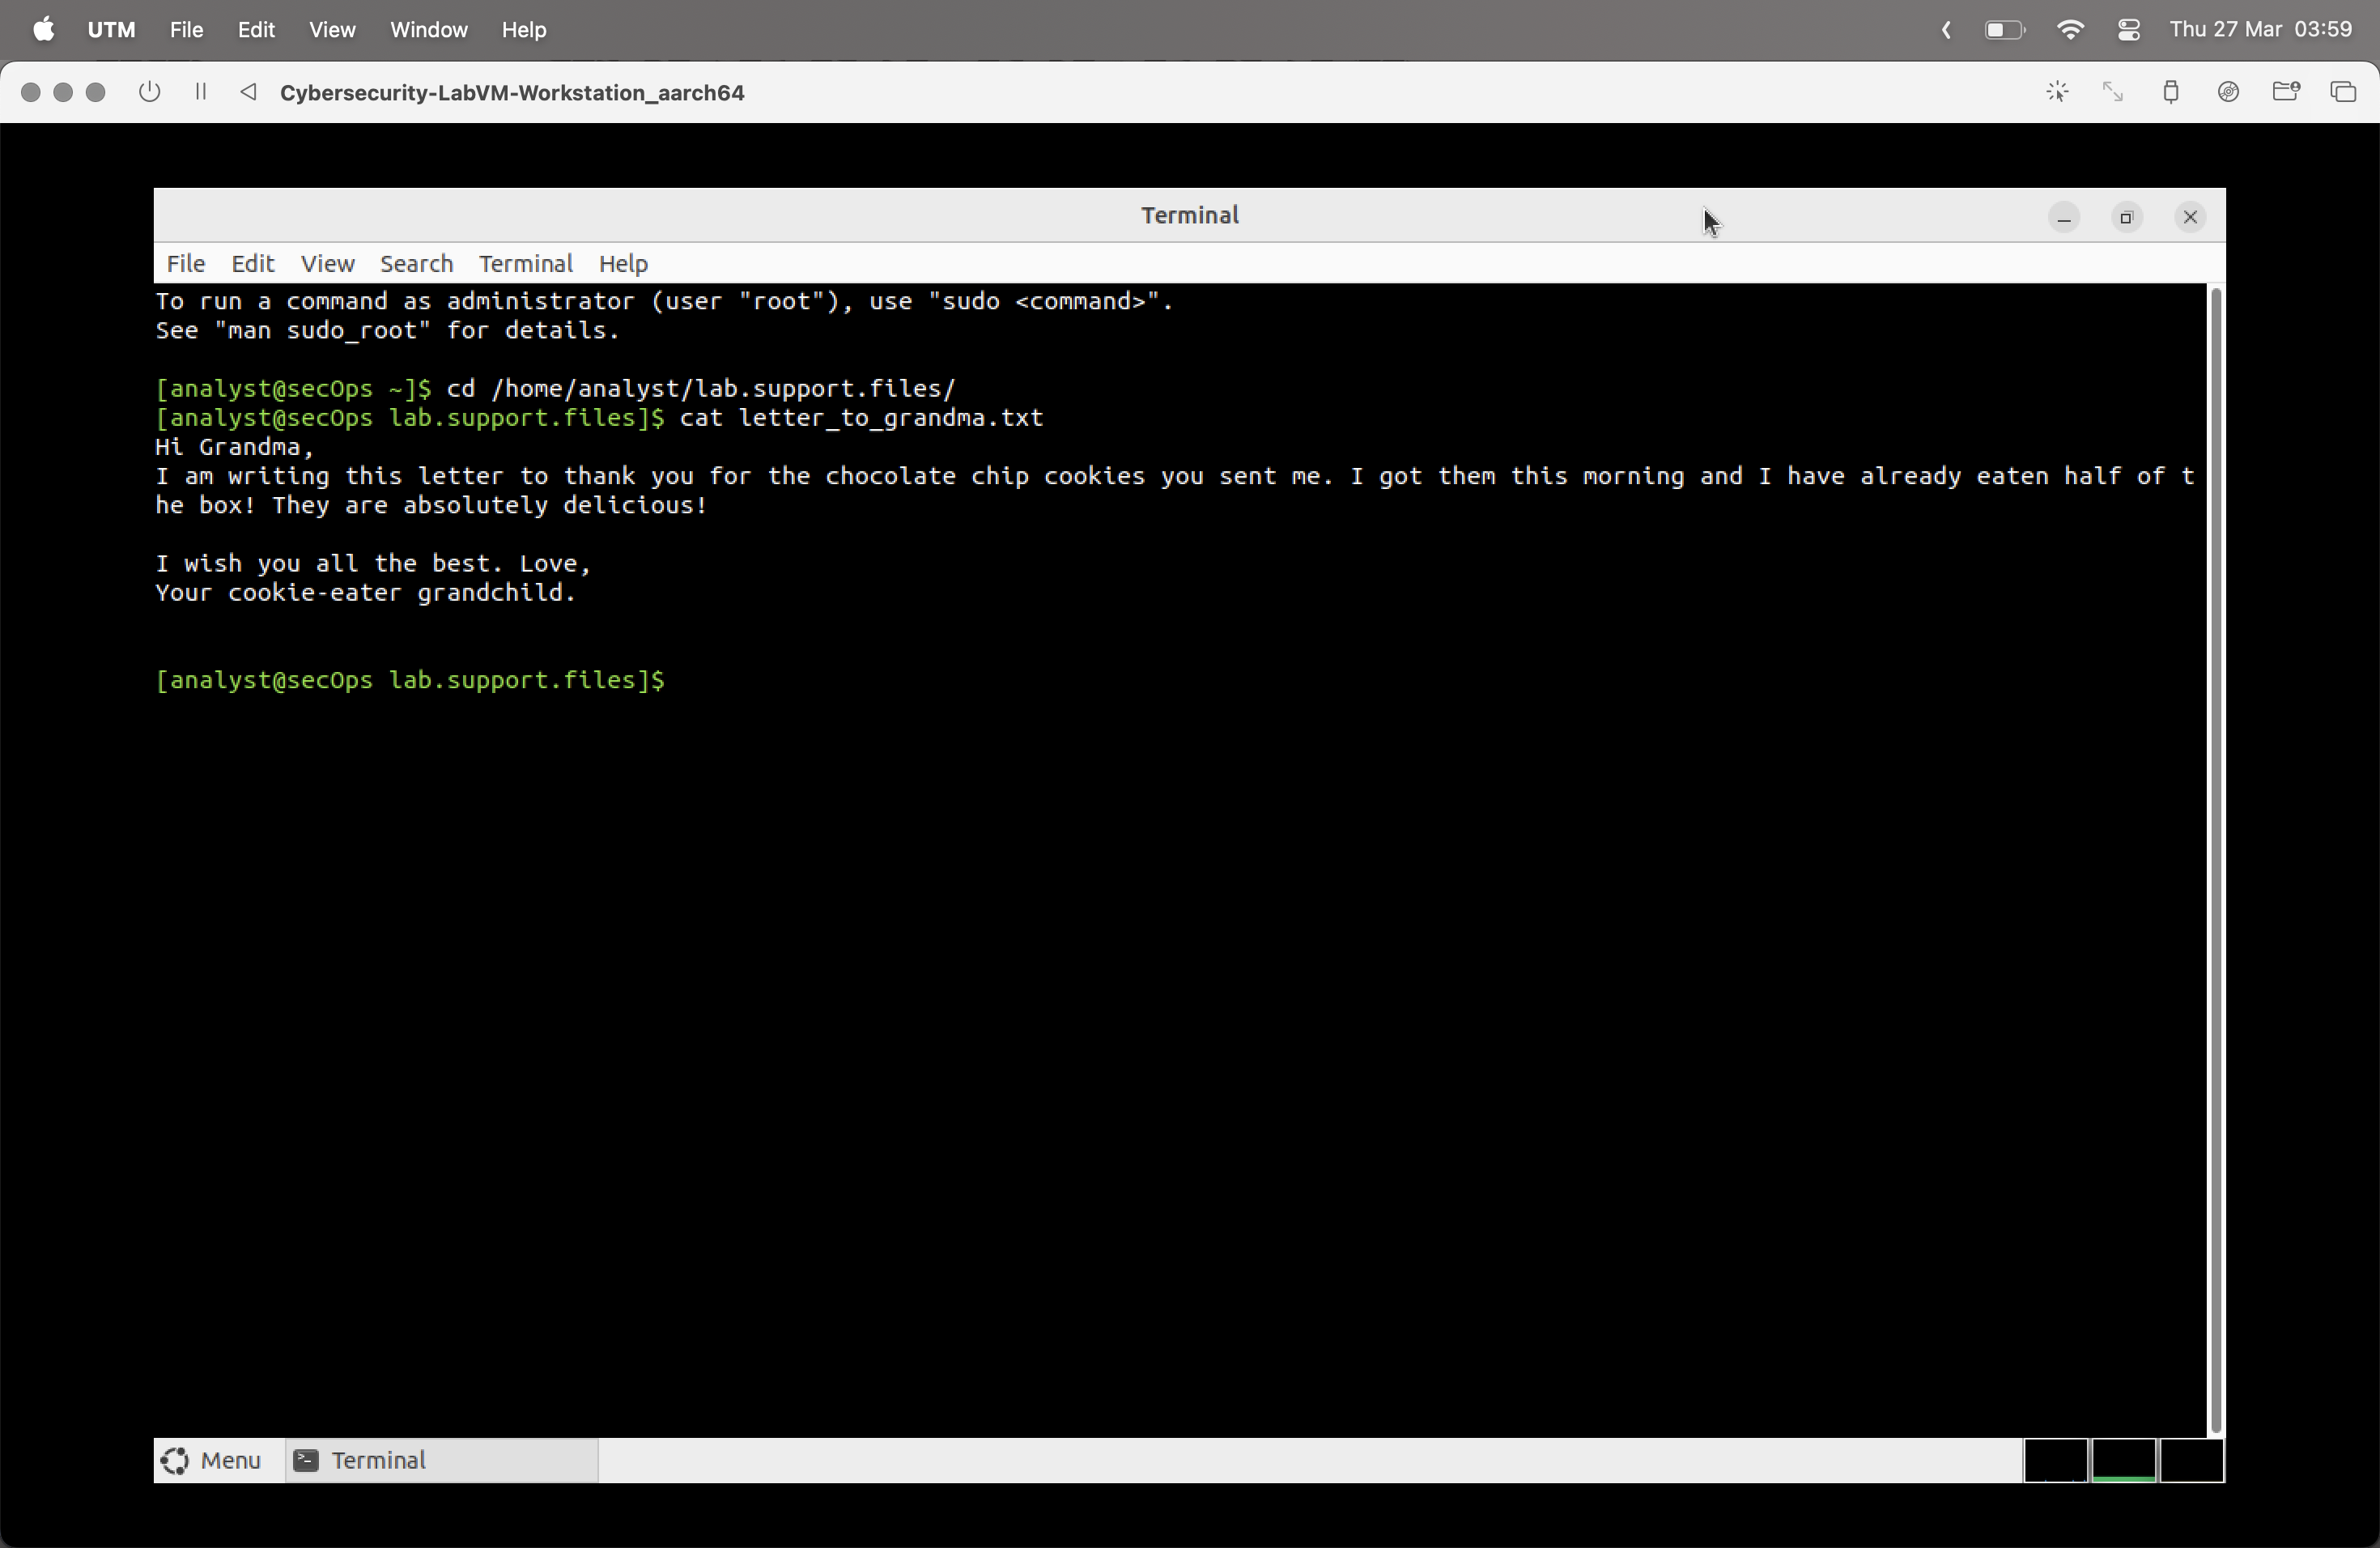
\includegraphics[width=0.8\textwidth]{lab3_text_file.png}
    \caption{Contents of letter\_to\_grandma.txt}
\end{figure}

Then I calculated its SHA-256 hash:

\begin{figure}[H]
    \centering
    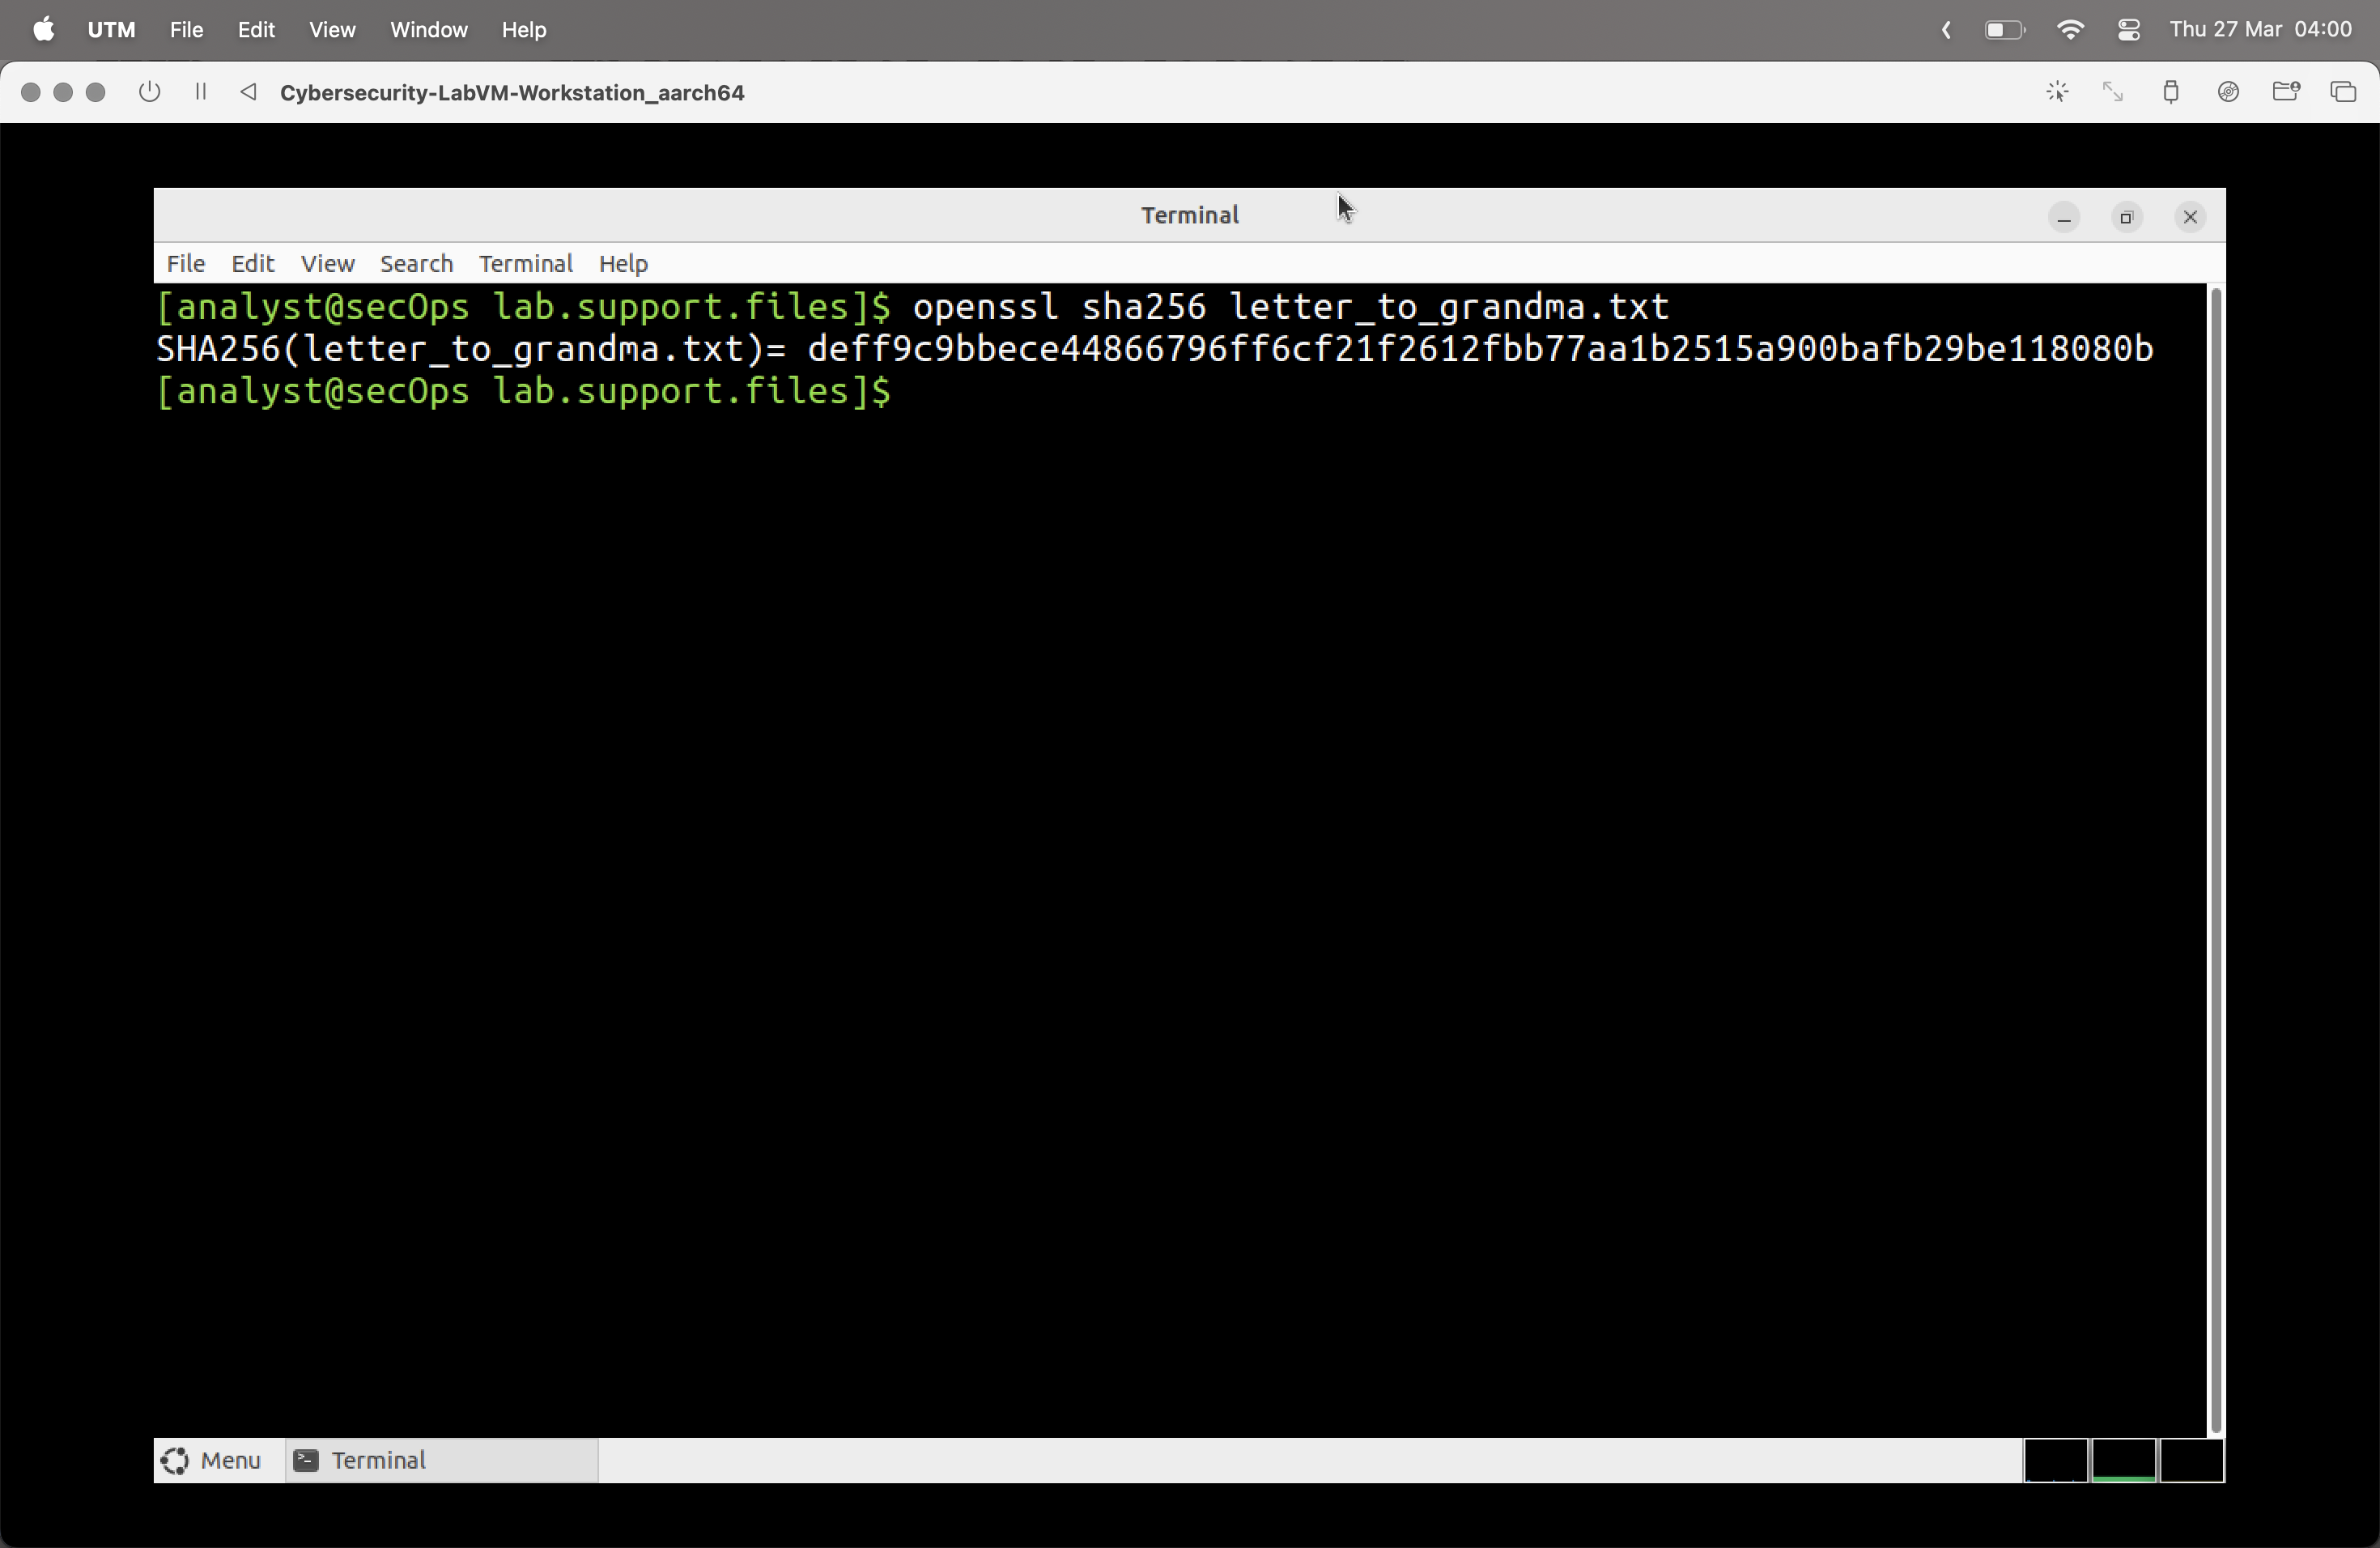
\includegraphics[width=0.8\textwidth]{lab3_initial_hash.png}
    \caption{SHA-256 hash of original text file}
\end{figure}

The original SHA-256 hash was:

\texttt{deff9c9bbece44866796ff6cf21f2612fbb77aa1b2515a900bafb29be118080b}

\subsubsection{Hash Comparison After File Modification}

I modified the text file by changing "Hi Grandma" to "Hi Grandpa" and recalculated the hash:

\begin{figure}[H]
    \centering
    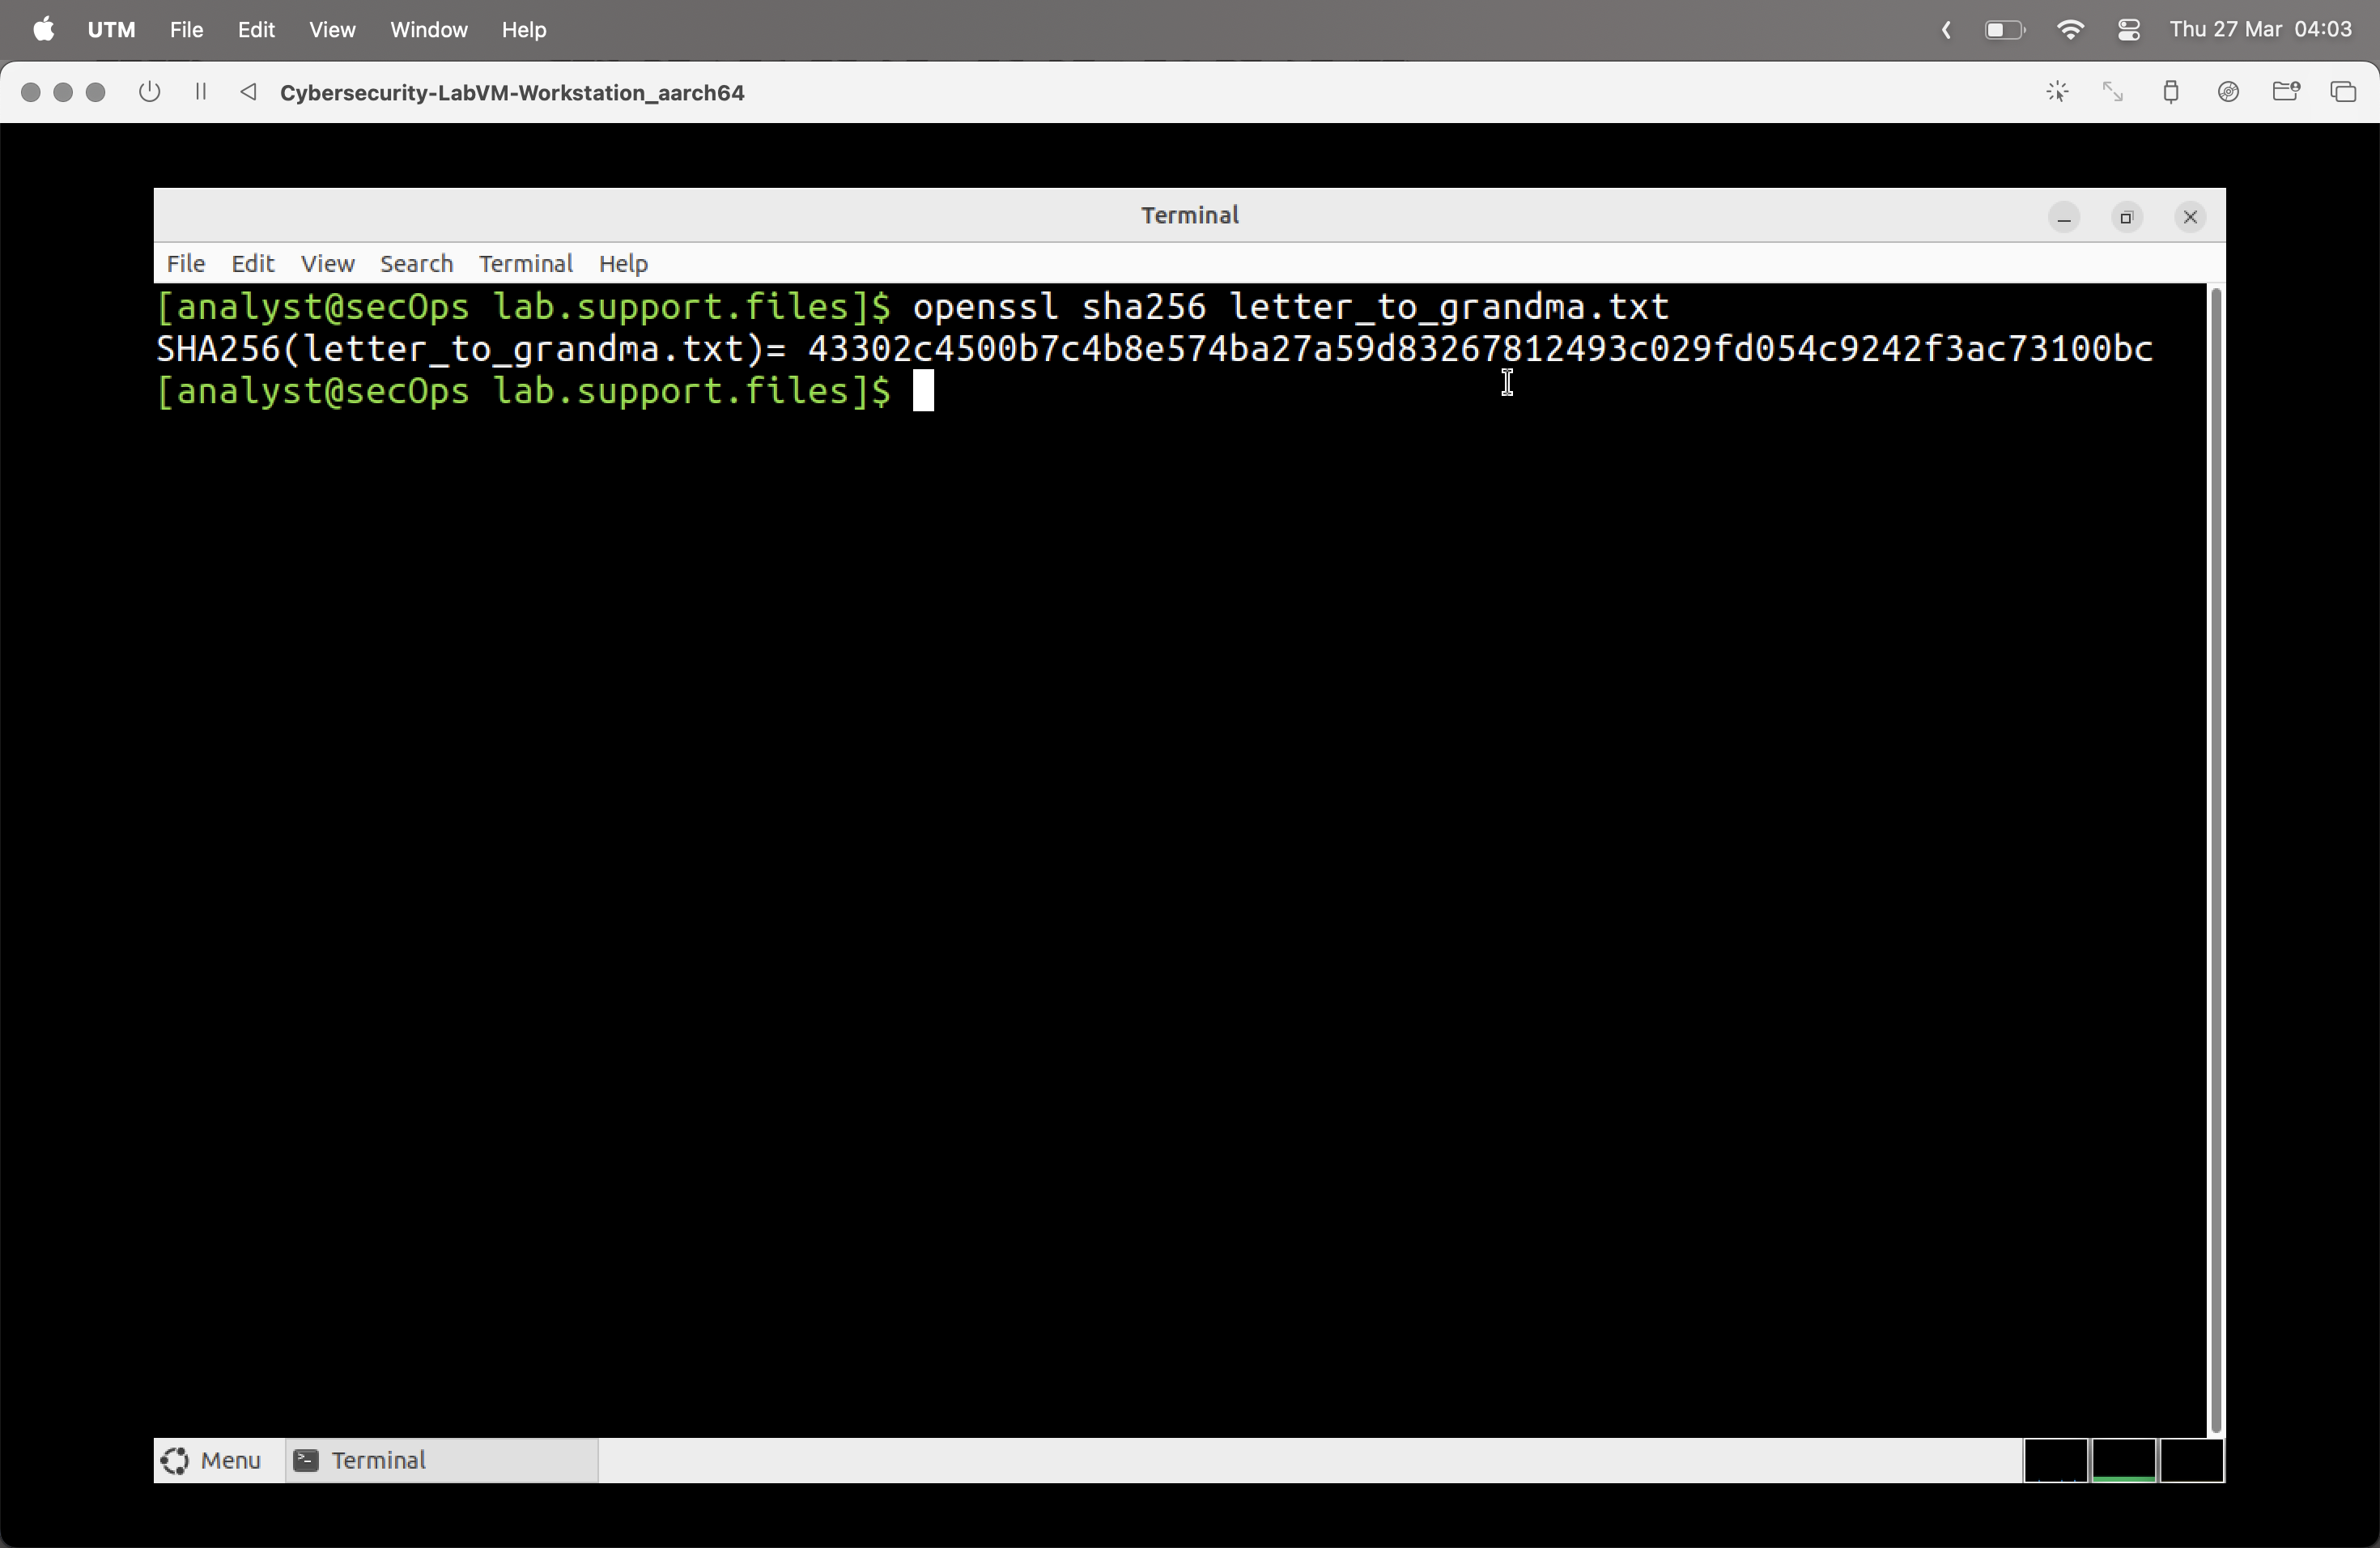
\includegraphics[width=0.8\textwidth]{lab3_modified_hash.png}
    \caption{SHA-256 hash of modified text file}
\end{figure}

The new SHA-256 hash was: 

\texttt{43302c4500b7c4b8e574ba27a59d83267812493c029fd054c9242f3ac73100bc}

\textbf{Analysis of Hash Differences:}
The two hashes are completely different despite changing only a single character in the text file. This demonstrates the "avalanche effect" of cryptographic hash functions, where even a minor change to the input results in a completely different hash output. There isn't a pattern or partial match between the hashes - they appear entirely unrelated, which is a critical security property of strong hash functions.

\subsubsection{Comparing Different Hash Algorithms}

I also generated SHA-512 hashes and compared results from different utilities:

\begin{figure}[H]
    \centering
    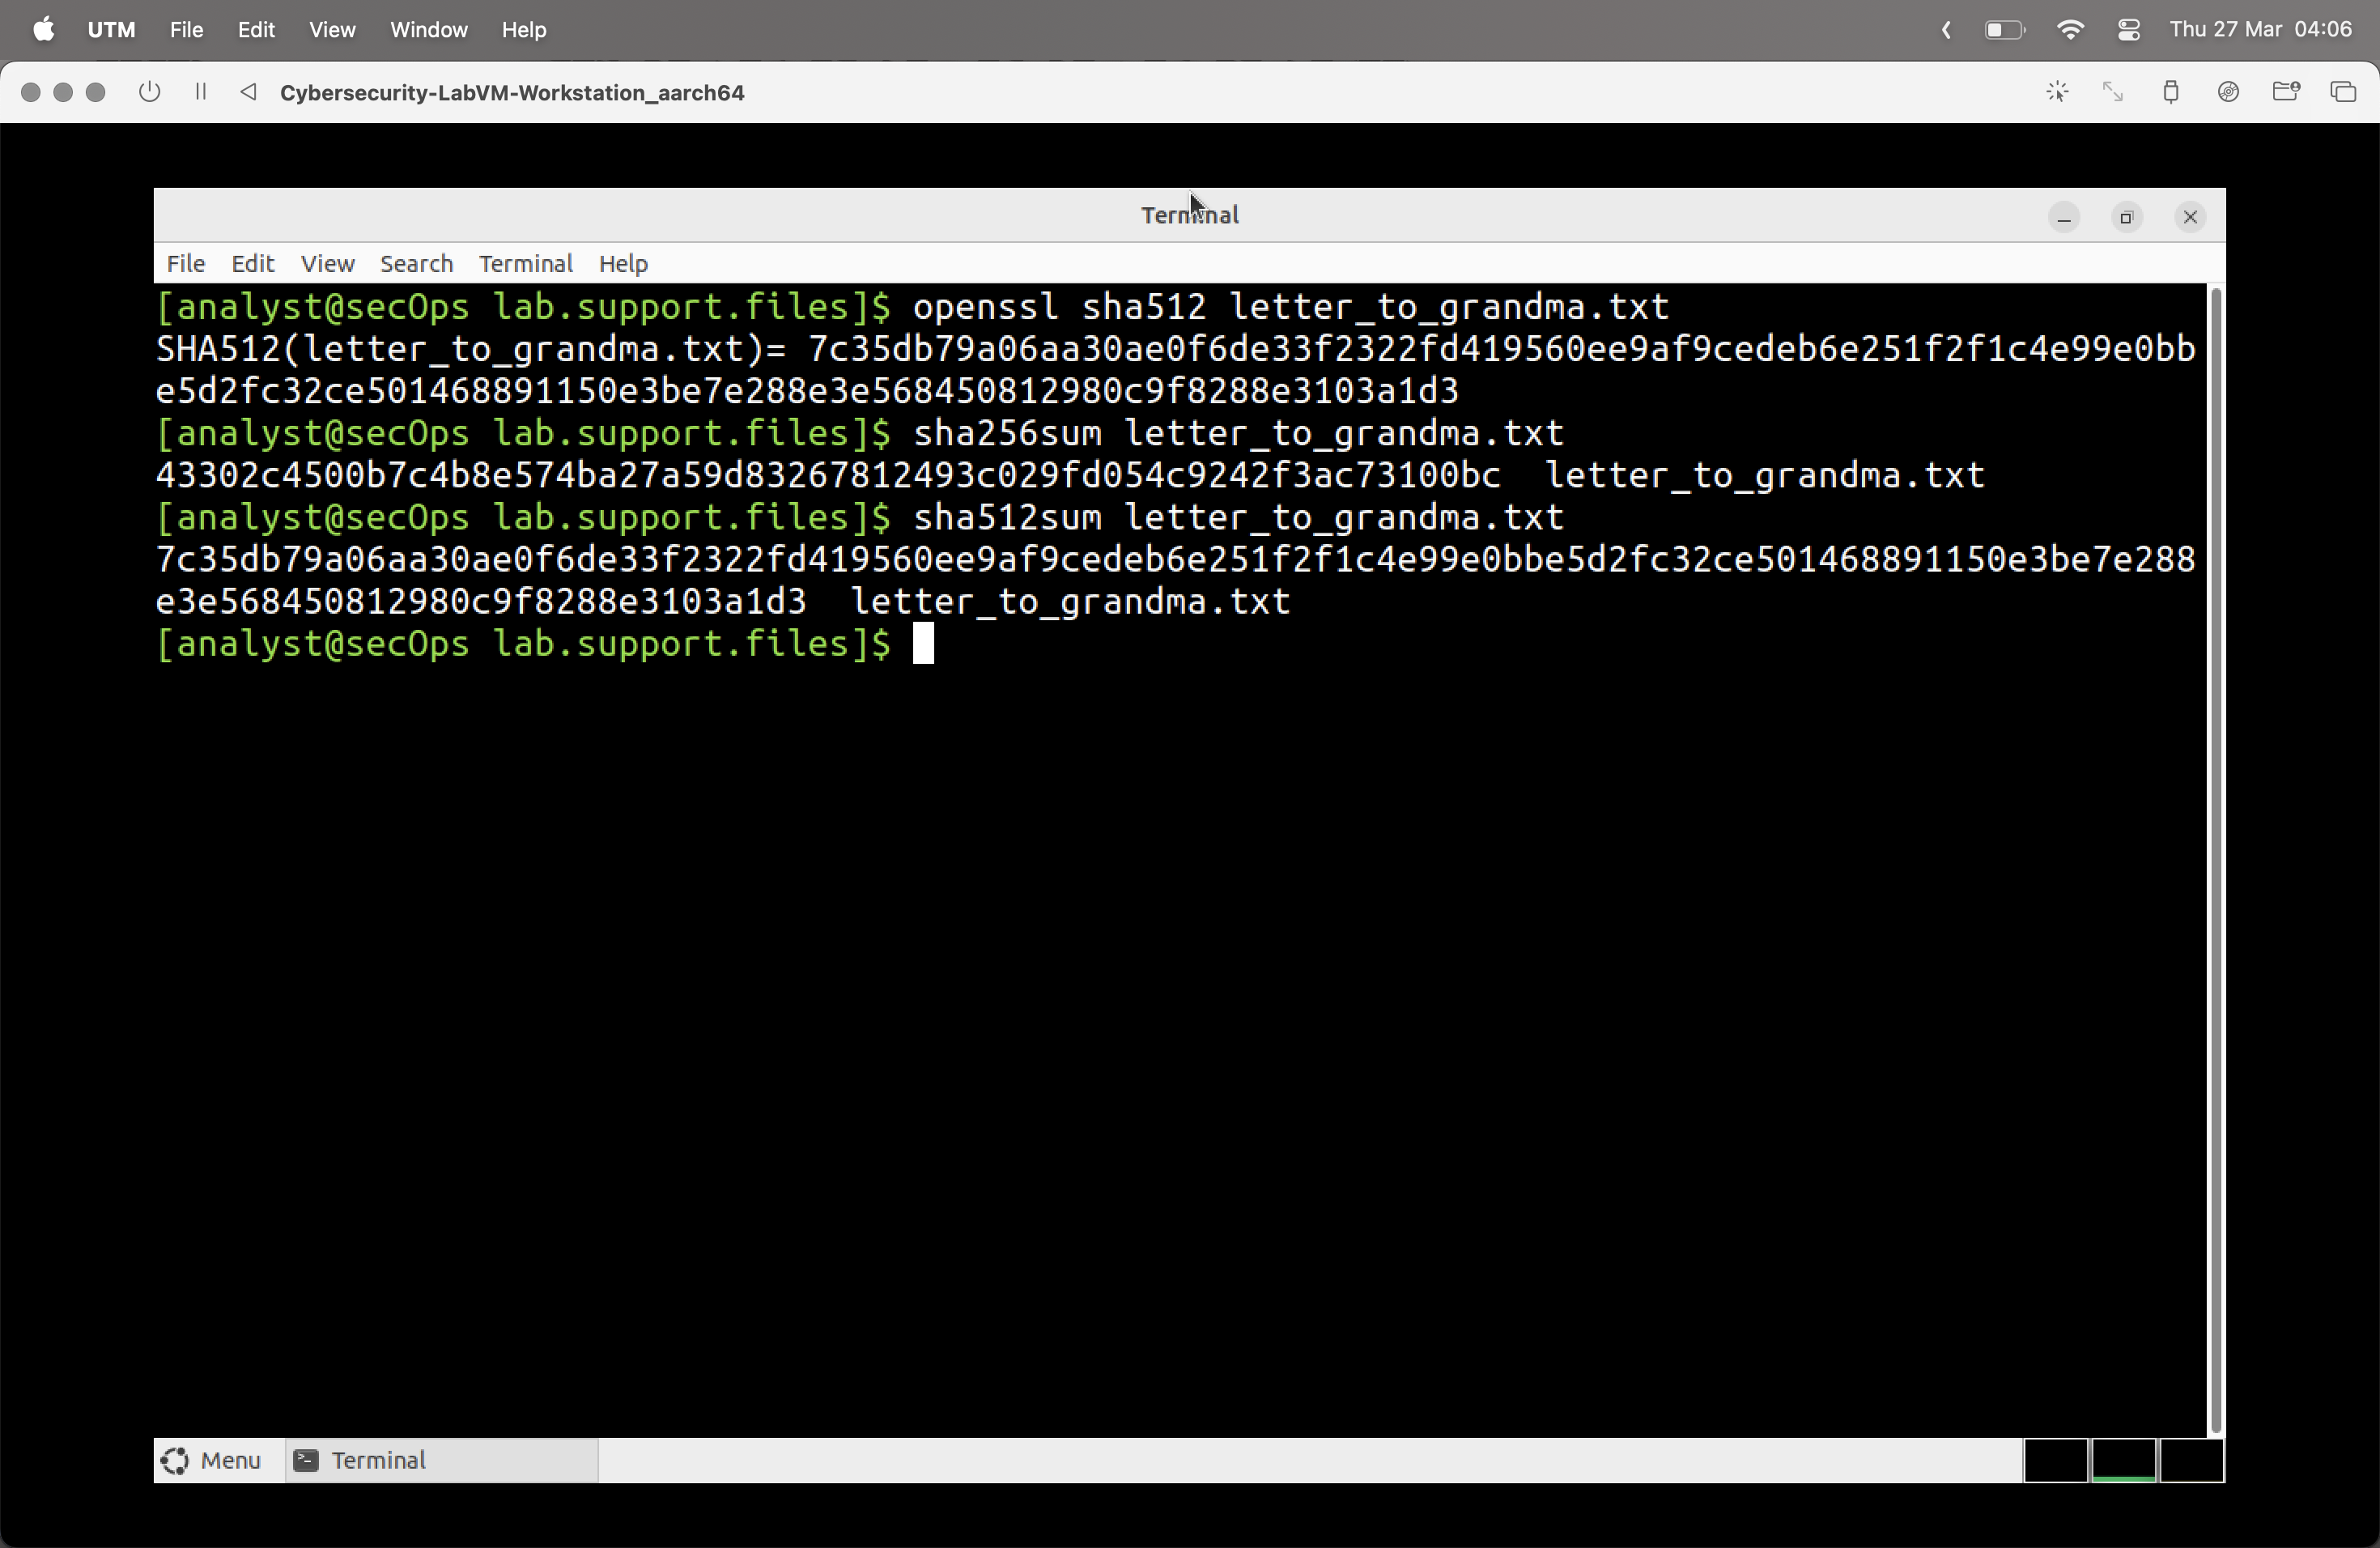
\includegraphics[width=0.8\textwidth]{lab3_multiple_hashes.png}
    \caption{SHA-512, sha256sum, and sha512sum results}
\end{figure}

\textbf{Comparison of Utilities:}
The hashes generated with \textbf{sha256sum} and \textbf{sha512sum} match exactly with those generated by OpenSSL's \textbf{openssl sha256} and \textbf{openssl sha512} commands. The only difference is in the output format - OpenSSL prefixes the hash with algorithm information and the filename, while the \textbf{sha256sum} and \textbf{sha512sum} utilities append the filename after the hash. This confirms that these tools implement the same standardized hash algorithms.

\newpage

\subsection{Part 2: Verifying Hashes}

In this part, I verified the integrity of a downloaded file by comparing its hash with a reference hash.

\subsubsection{Hash Verification Process}

I first viewed the contents of the reference hash file:

\begin{figure}[H]
    \centering
    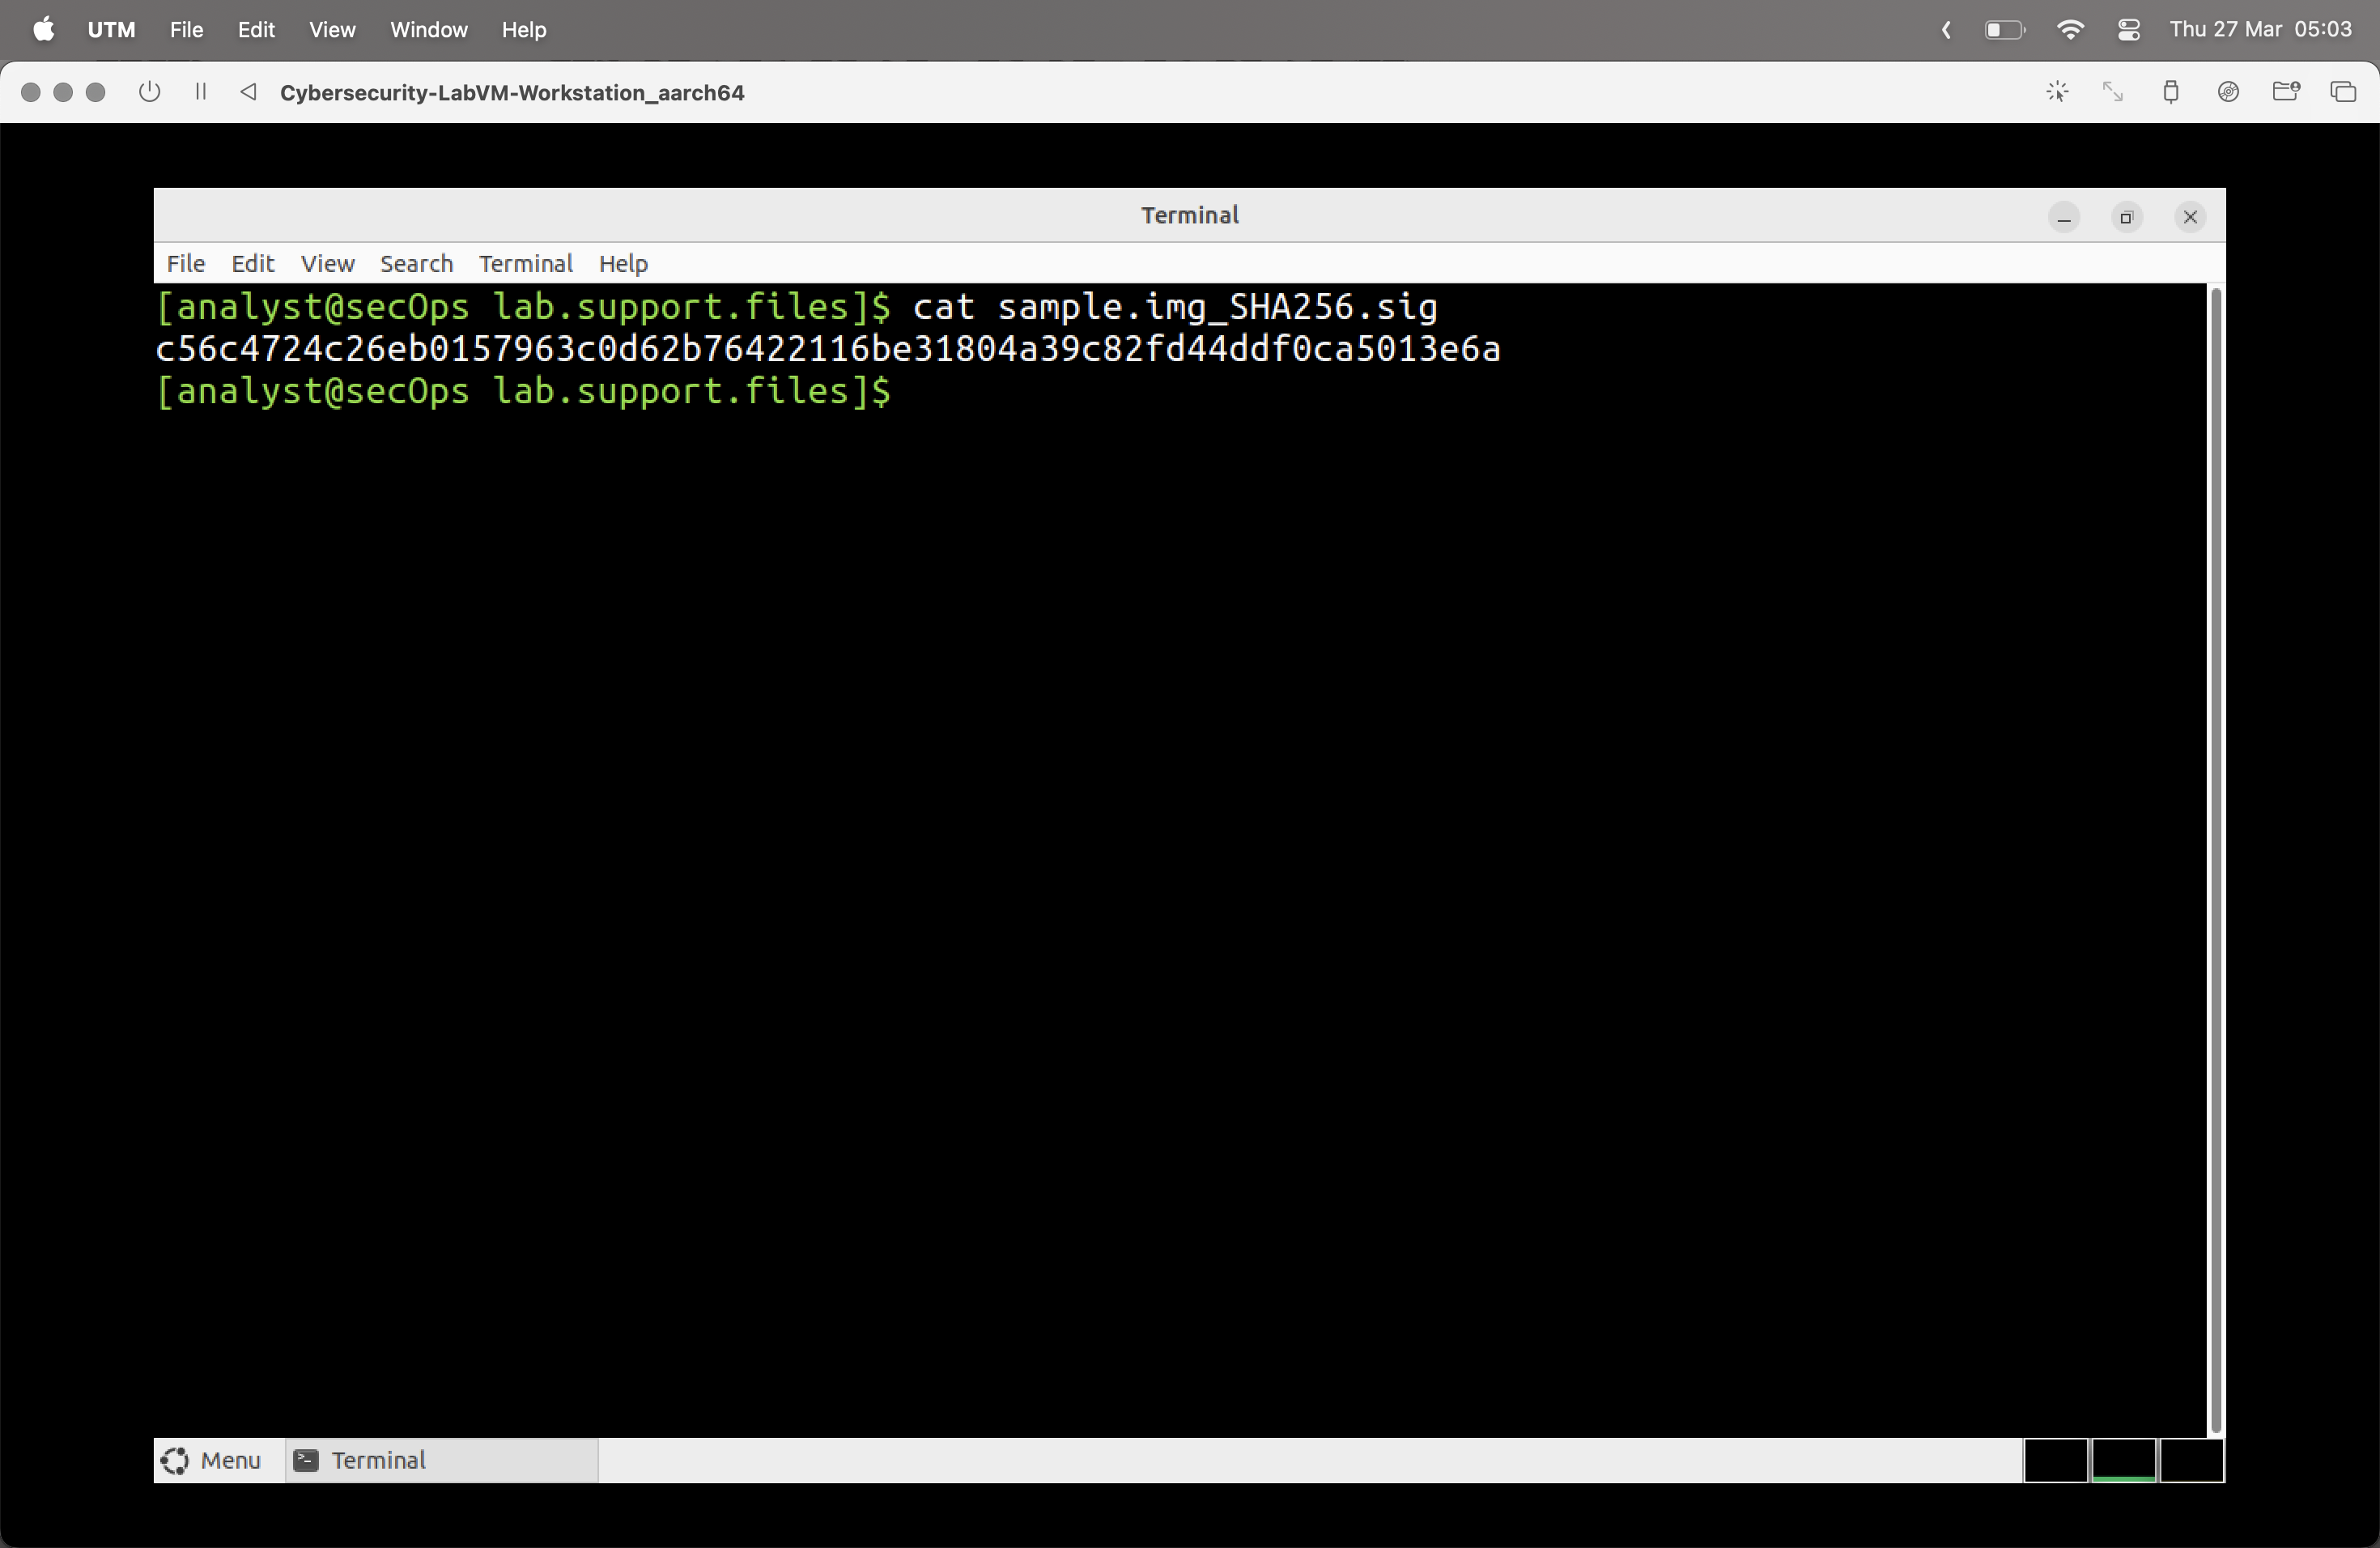
\includegraphics[width=0.8\textwidth]{lab3_reference_hash.png}
    \caption{Contents of sample.img\_SHA256.sig file}
\end{figure}

Then I calculated the SHA-256 hash of the sample file:

\begin{figure}[H]
    \centering
    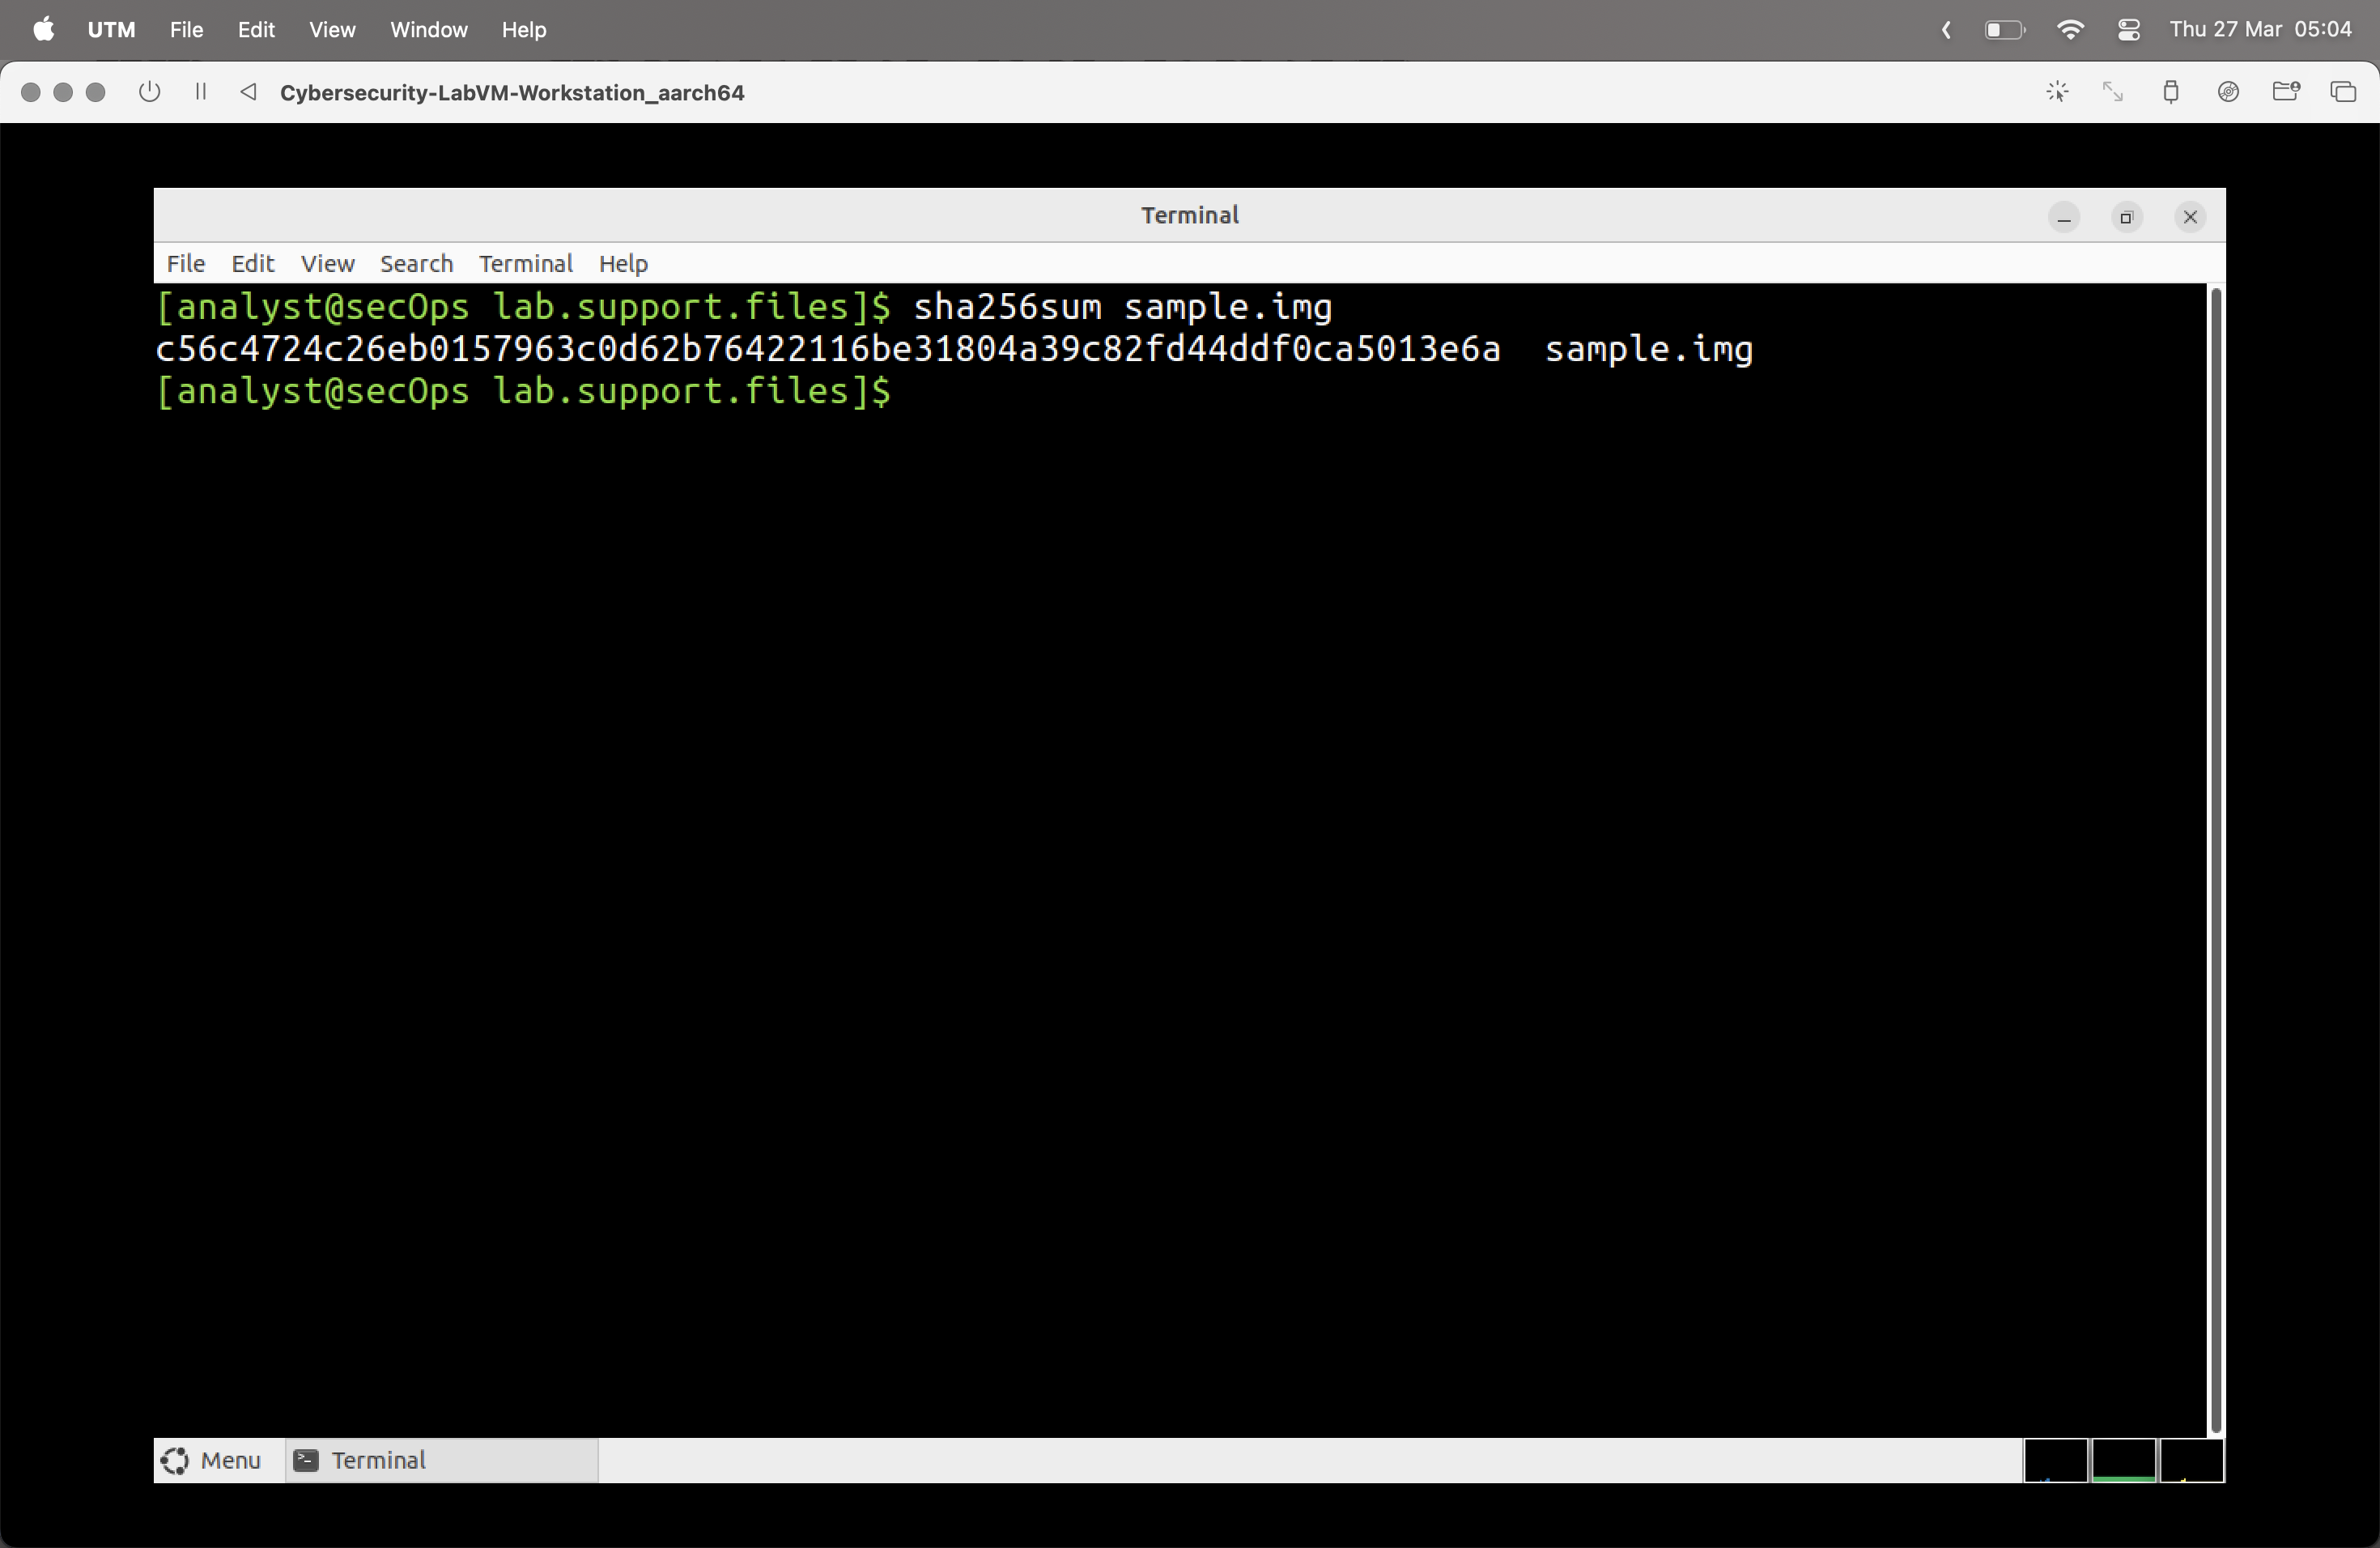
\includegraphics[width=0.8\textwidth]{lab3_sample_hash.png}
    \caption{SHA-256 hash of sample.img file}
\end{figure}

\textbf{Integrity Verification Results:}
The SHA-256 hash of sample.img calculated using sha256sum is:
\texttt{c56c4724c26eb0157963c0d62b76422116be31804a39c82fd44ddf0ca5013e6a}

This hash exactly matches the reference hash in sample.img\_SHA256.sig, confirming that the sample.img file was downloaded without errors or tampering. This verification process demonstrates how hash functions can be used to verify file integrity after transmission or storage.

\subsection{Lab 3 Conclusion}
Through this lab, I gained practical experience with cryptographic hash functions and their applications:

\begin{itemize}
    \item I observed how hash functions produce completely different outputs even with minimal input changes
    \item I compared different hash algorithms (SHA-256 vs. SHA-512) and utilities
    \item I applied hashing to verify file integrity, demonstrating a real-world security application
\end{itemize}
This practical understanding of hashing is essential for various security applications, including:
\begin{itemize}
    \item Data integrity verification
    \item Password storage (when combined with salting)
    \item Digital signatures
    \item File and message authentication
\end{itemize}

\end{document}